\documentclass[
  reprint,
  amsmath,
  amssymb,
  aps,
  pra,
  nofootinbib,
  superscriptaddress,
  floatfix
]{revtex4-2}

\usepackage[T1]{fontenc}
\usepackage{lmodern}
\usepackage{newunicodechar}
\newunicodechar{’}{'}
\usepackage{graphicx}
\graphicspath{{../../}{}}
\usepackage{capt-of} % \captionof for non-floating figures (used with widetext)
\usepackage{booktabs}
\usepackage{bm}
\usepackage{mathtools}
\usepackage{amsthm}
\usepackage{xcolor}
\usepackage{hyperref}

\newcommand{\placeholder}[1]{\textcolor{red!70!black}{\ifmmode\left[#1\right]\else\textsf{[#1]}\fi}}
\newcommand{\tentative}[1]{\textcolor{red!70!black}{#1}}
\newcommand{\structlabel}[1]{\noindent\mbox{\tentative{#1.}}~}
\newcommand{\Oset}{\mathcal{O}}
\newcommand{\Gset}{\mathcal{G}}
\newcommand{\Rset}{\mathcal{R}}
\newcommand{\Sset}{\mathcal{S}}
\newcommand{\Hcal}{\mathcal{H}}
\newcommand{\Bcal}{\mathcal{B}}
\newcommand{\Ocal}{\mathcal{O}}
\newcommand{\Ucal}{\mathcal{U}}
\newcommand{\Jcal}{\mathcal{J}}
\newcommand{\Pcal}{\mathcal{P}}
\newcommand{\Dcal}{\mathcal{D}}
\newcommand{\Mcal}{\mathcal{M}}
\newcommand{\Wcal}{\mathcal{W}}
\newcommand{\dd}{\mathrm{d}}
\newcommand{\ii}{\mathrm{i}}
\newcommand{\ee}{\mathrm{e}}
\newcommand{\TR}{\mathrm{TR}}
\newcommand{\ex}{\mathrm{ex}}
\newcommand{\ctrl}{\mathrm{ctrl}}
\newcommand{\stat}{\mathrm{stat}}
\newcommand{\dyn}{\mathrm{dyn}}
\newcommand{\drv}{\mathrm{drv}}
\newcommand{\obs}{\mathrm{obs}}
\newcommand{\stay}{\mathrm{stay}}
\newcommand{\app}{\mathrm{append}}
\newcommand{\ablate}{\mathrm{ablate}}
\newcommand{\Var}{\operatorname{Var}}
\newcommand{\Tr}{\operatorname{Tr}}
\newcommand{\Top}{\operatorname{Top}}
\newcommand{\argminp}{\mathop{\mathrm{arg\,min}}}
\newcommand{\argmaxp}{\mathop{\mathrm{arg\,max}}}
\newcommand{\proj}{\mathrm{proj}}
\newcommand{\diag}{\mathrm{diag}}
\newcommand{\CVaR}{\operatorname{CVaR}}
\newcommand{\softmax}{\operatorname{softmax}}
\newcommand{\hh}{\mathrm{HH}}
\newcommand{\phmax}{n_{\mathrm{ph,max}}}
\newcommand{\twq}{\mathrm{2Q}}
\newcommand{\eps}{\varepsilon}
\newcommand{\ket}[1]{|#1\rangle}
\newcommand{\bra}[1]{\langle #1|}
\newcommand{\braket}[2]{\langle #1|#2\rangle}
\newcommand{\expval}[1]{\langle #1\rangle}
\newcommand{\metrichead}[1]{\makebox[0.061\textwidth][c]{#1}}
\newcommand{\archmetrichead}[1]{\makebox[0.040\textwidth][c]{#1}}
\newcommand{\inlinetablecaption}[2]{%
  \par\addvspace{1.6ex}%
  \captionof{table}{#2\label{#1}}%
  \par\addvspace{0.8ex}%
}
\newenvironment{schurlemma}[1][]
{\par\medskip\noindent\textbf{Lemma}\if\relax\detokenize{#1}\relax\else\ (#1)\fi.\space\itshape}
{\par\medskip}
\newenvironment{schurassumption}[1][]
{\par\medskip\noindent\textbf{Assumption}\if\relax\detokenize{#1}\relax\else\ (#1)\fi.\space}
{\par\medskip}
\newenvironment{schurtheorem}[1][]
{\par\medskip\noindent\textbf{Theorem}\if\relax\detokenize{#1}\relax\else\ (#1)\fi.\space\itshape}
{\par\medskip}
\newenvironment{schurremark}[1][]
{\par\medskip\noindent\textbf{Remark}\if\relax\detokenize{#1}\relax\else\ (#1)\fi.\space}
{\par\medskip}


\begin{document}

\title{Geometry- and Cost-Aware ADAPT Ansatz Construction for Mixed Fermion--Boson Hamiltonians}

\author{Jake Strobel}
\author{Jacopo Simoni}
\author{Gabrielle Riva}
\author{Yuan Ping}
\affiliation{University of Wisconsin--Madison}

\date{\today}



\begin{abstract}
Mixed fermion--boson Hamiltonians combine electronic correlation with truncated bosonic motion, producing compact few-site benchmarks whose informative observables are already difficult for noisy quantum processors because two-qubit depth, measurement burden, and variational refit cost grow rapidly.  We present SNAKE, a geometry- and cost-aware ADAPT gate-selection procedure for ground-state ansatz construction.  Candidate generators are promoted to candidate--position records and scored through lower-confidence Fubini--Study trust-region gain, hardware and measurement cost penalties, tangent novelty, Schur-refit reranking, batching, beam continuation, and rollback-safe generator ablation.  For the two-site one-dimensional Hubbard--Holstein lattice in the weak-coupling regime, SNAKE obtains a \(37.4\%\) smaller energy error than the best ADAPT competitor, while reducing two-qubit count by \(87.6\%\), two-qubit depth by \(94.5\%\), total circuit depth by \(80.9\%\), and the shot-count proxy by \(69.5\%\); in the strong-coupling regime, at matched energy error relative to Geo-ADAPT, SNAKE reduces two-qubit count by \(45.8\%\), two-qubit depth by \(44.5\%\), total circuit depth by \(46.8\%\), and the shot-count proxy by \placeholder{XX\%}. We show similar improvements for fermion models such as Hubbard, and boson models such as the spin-boson.
\end{abstract}

\maketitle







\section{Introduction}

\structlabel{Problem, Hamiltonian, importance of solving it}
Mixed fermion--boson Hamiltonians describe many-body systems in which electronic correlation, lattice vibrations, and electron--phonon interactions determine the relevant eigenstates and observables \cite{Hubbard1963,Holstein1959a,Holstein1959b}. These include lattice models such as Hubbard--Holstein and spin--boson Hamiltonians, as well as molecular, vibronic, and electron--phonon models in which electronic degrees of freedom are coupled to discrete or truncated bosonic modes. An important problem in condensed-matter, molecular physics, and quantum-simulation applications is to approximate low-energy states of the truncated Hilbert space and use them to compute site-resolved densities and occupations, correlation effects, mode-resolved bosonic occupation and electron-phonon interactions. These low-energy-state calculations also provide the starting point for variational real-time dynamics and subspace-based excited-state spectra \cite{LiBenjamin2017VQS,Yuan2019VQS,McClean2017QSE}.

Classical solvers are effective for small systems, but their cost increases rapidly with the number of  orbitals, lattice sites, and retained bosonic levels.  Dense exact diagonalization scales cubically with the truncated Hilbert space dimension \cite{Weisse2008}; sparse eigensolvers reduce the cost but remain controlled by Hamiltonian sparsity and the number of targeted low-energy states \cite{Schollwock2011}; tensor-network costs can grow with the entanglement-controlled bond dimension and the bosonic local dimension \cite{Schollwock2011}; and quantum Monte Carlo can encounter sign- or phase-problem scaling \cite{Troyer2005}. Qubit encodings reduce these difficulties by representing an \(N\)-level local bosonic cutoff with \(O(\log N)\) qubits \cite{Sawaya2020,Li2023}. On current quantum processors, however, the bottleneck shifts to ansatz construction, circuit compilation and repeated expectation value estimation. Entangling depth and number of measurements, therefore, determine whether a compact encoded representation can be turned into a real executable and produce accurate results for the observables of interest.

We consider Hamiltonians with the following general form\cite{Dutta2024BosonicChemistry,Peng2025BosonHamiltonians}
\begin{align}
H&=H_f+H_b+H_{fb},
\nonumber\\
H_f&=\sum_{pq}h_{pq}c_p^\dagger c_q
+\frac12\sum_{pqrs}V_{pqrs}c_p^\dagger c_q^\dagger c_s c_r,
\nonumber\\
H_b&=\sum_{\mu}\omega_\mu b_\mu^\dagger b_\mu+H_b^{\rm nl},
\nonumber\\
H_{fb}&=\sum_{\mu}X_\mu^{(b)}F_\mu^{(f)}
+\sum_{\mu}P_\mu^{(b)}G_\mu^{(f)},
\label{eq:general_fb_terms_static}
\end{align}
where $X_\mu^{(b)}=b_\mu^\dagger+b_\mu$ and $P_\mu^{(b)}=\ii(b_\mu^\dagger-b_\mu)$, while $F_\mu^{(f)}$ and $G_\mu^{(f)}$ denote fermionic density or orbital-transition operators coupled to the bosonic displacement and momentum operators, respectively. Hubbard, Hubbard--Holstein, boson-only, spin-boson, molecular electronic, and vibronic Hamiltonians are treated as limiting cases, with specific forms given in Appendix~\ref{app:hamiltonian_families}. For qubit representation, we use Jordan--Wigner fermionic encodings, together with binary bosonic encodings and fixed blocked fermionic/bosonic registers for each benchmark instance.

\paragraph*{Current status}
Ground-state calculations for electronic structure and electron-phonon coupled systems on a quantum processor are commonly formulated as Rayleigh--Ritz minimizations on a parameterized trial wave function\cite{Peruzzo2014,McClean2016,Kandala2017},
\begin{equation}
E(\boldsymbol{\theta})=
\bra{\psi_{\rm ref}}U^\dagger(\boldsymbol{\theta})HU(\boldsymbol{\theta})\ket{\psi_{\rm ref}},
\label{eq:rayleigh_static}
\end{equation}
where \(\ket{\psi_{\mathrm{ref}}}\) is typically a simple and physically motivated reference state, and $\boldsymbol{\theta}=(\theta_1,\ldots,\theta_n)$ is the parameter vector associated with the wave function ansatz. For mixed fermion--boson systems, we use a Hartree-Fock determinant for the electronic subspace, tensored with a bosonic reference state, usually taken as the phonon vacuum, \(\ket{\psi_{\mathrm{ref}}}=\ket{\mathrm{HF}}\otimes\ket{0_1\,0_2\,\cdots\,0_{\mathrm{M}}}\), where \(M\) is the number of retained phononic modes. The main ansatz choice is whether the unitary \(U(\boldsymbol{\theta})\) is fixed before the calculation or constructed adaptively. Fixed-structure variational circuits prescribe the full ansatz in advance, fixing the parameter count, number of entanglers and nominal circuit depth. ADAPT-style methods instead grow \(U(\boldsymbol{\theta})\) iteratively by selecting generators from a predefined pool \(\mathcal{G}\) using energy-gradient information\cite{Grimsley2019,Tang2021,Yordanov2021}. At ADAPT iteration \(k\), let \(\boldsymbol{\theta}_k\) denote the current parameter vector. The appended generator is chosen as
%\(A^\star\) is selected from a predefined pool \(\mathcal G\) by maximizing the local energy-gradient objective,
\begin{equation}
A_k^\star=\arg\max_{A\in\mathcal G}
\left|
\left.
\partial_{\theta_{n_k}}E\!\left(e^{\theta_{n_k} A}U_k(\boldsymbol{\theta}_{k-1})\ket{\psi_{\mathrm{ref}}}\right)
\right|_{\theta_{n_k}=0}
\right|\,,
\end{equation}
where the $E(\ket{\psi(\boldsymbol{\theta})})$ is the expectation value of the Hamiltonian on the trial wave function $\ket{\psi(\boldsymbol{\theta})}$. The new generator is then appended to the ansatz,
\begin{equation}
U_{k+1}(\boldsymbol{\theta}_{k})=e^{\theta_{n_k} A_k^\star}U_k(\boldsymbol{\theta}_{k-1}).
\end{equation}
In either case, the parameterization update rule is
\begin{equation}
\label{eq:theta_opt}
\boldsymbol{\theta}^\star=\arg\min_{\boldsymbol{\theta}}E(\boldsymbol{\theta})\,.
\end{equation}
%
Several ADAPT variants follow different strategies to select the generators. TETRIS-ADAPT improves compactness by batching compatible qubit-disjoint generators\cite{Anastasiou2024}, CEO-ADAPT uses coupled-exchange operator sequencing\cite{Ramoa2025}; Overlap-ADAPT modifies the append criterion using tangent-direction information\cite{Feniou2023}. Other works introduce second-order information to improve convergence\cite{Grimsley2023ADAPT} or utilize Hessian information to warm-start parameters across iterations and reduce optimizer overhead\cite{Ramoa2025HessianRecycling}.\\
Geo-ADAPT-VQE replaces the Euclidean \(\theta\)-space metric with a state-space Fubini--Study metric, permitting generator insertion rather than append-only growth\cite{Sohail2026GeoADAPT}. Prune ADAPT removes previously selected generators using a criterion based on amplitude and iteration-history\cite{Vaquero2025PrunedADAPT}.

\paragraph*{Limitations with current approaches}
Despite these advances, current adaptive strategies leave several unresolved issues. Standard ADAPT, Qubit-ADAPT, and qubit-excitation ADAPT rely on first-order energy gradients to select generators\cite{Grimsley2019,Tang2021,Yordanov2021} and can therefore be sensitive to gradient plateaus or local-minima\cite{Feniou2023,Grimsley2023ADAPT}.\\
TETRIS-ADAPT reduces depth by adding several compatible high-gradient operators in one iteration, but it inherits the same first-order selection criterion\cite{Anastasiou2024}. Second-order derivative information can help escape first-order stagnation\cite{Ramoa2025HessianRecycling}, but derivative scores defined directly in parameter-space can be sensitive to the chosen parametrization rather than to changes in the Hilbert space state vector\cite{ProvostVallee1980,Stokes2020QNG}. Geo-ADAPT partially addresses the problem by using the Fubini--Study metric; however, its inverse can become ill-conditioned or rank-deficient in heterogeneous operator pools, where distinct generators can induce duplicate or nearly redundant tangent directions\cite{Sohail2026GeoADAPT}. The integration of Fubini--Study/QIM scoring with second-order curvature, batching, and pruning remains an open additional complexity.%this is part of what snake does

Three global shortcomings remain across these variants: (1) an iteration-independent shot budget can overpay early and underpay late stage due to the iteration-dependent decrease in candidate signal-to-noise ratio \cite{Ikhtiarudin2025ShotEfficient}, (2) absent a cost penalty, a candidate operator with a marginal gradient advantage can score higher despite having arbitrarily greater circuit-burden, and (3) no method currently considers whether the candidate’s tangent direction has a nonzero residual component after projection against the locally reoptimized current-ansatz tangent space.


\structlabel{Solution strategy}
To avoid parameter-coordinate sensitivity and unreduced inverse pool-metric dependence, SNAKE evaluates operator-position records with a regularized Fubini--Study metric \cite{Sohail2026GeoADAPT}. SNAKE incorporates a second-order Taylor model into the energy-gradient objective of Eq. (3), but constrains the maximization to a geometric trust region \cite{Nocedal2006TrustRegion}. SNAKE allows a local-reparameterization window to avoid full-ansatz reparameterization after each admission; this window is the coordinate set used by the Schur reduction. The reduced Schur model ranks candidates by residual trust-region gain after accounting for coupling between existing ansatz tangent directions and candidate tangents under mutual reparameterization through a regularized Hessian treatment.

Then, degenerately scored candidates can be admitted jointly via TETRIS-ADAPT--like treatment\cite{Anastasiou2024}, conditional on tangent nonredundancy. Under degenerate batch candidacy. SNAKE borrows Lowerre-style beam search to branch candidate circuits in parallel, with branch pruning upon dominance or budget pressure \cite{Lowerre1976Beam}.

To reduce persistent circuit cost, SNAKE enables a nested Schur ladder that analytically qualifies local recoverability under generator ablation \cite{Vaquero2025PrunedADAPT}. SNAKE further down-regulates circuit burden by an inter-pool variance weighting within the gradient-descent objective, penalizing candidate scoring by proxied two-qubit, circuit-depth, and shot burden \cite{Verteletskyi2020CliqueCover,Yen2020CompatibleMeasurements,Ikhtiarudin2025ShotEfficient}.

SNAKE uses a four-part generator scoring sequence with intermittent shortlisting based on Pauli support and commutation status. This shortlisting limits shot overhead by restricting expensive metric, curvature, and Schur evaluations to candidates that survive algebraically partitioned prior-phase scoring.

The generator-position record set magnitude and scores are iteration-dependently weighted. As the ansatz matures, local-reparameterization windows contract, shortlist pressure increases, expensive phases eventually retire, and shot counts rise to combat candidate signal-to-noise decreases.

Finally, SNAKE is evaluated on fermionic, bosonic, and mixed fermion--boson Hamiltonians. Fixed-structure VQE has been applied to bosonic qumode/model Hamiltonians and to bosonic or supersymmetric high-energy matrix models \cite{Dutta2026QumodeVQE,Rinaldi2022MatrixModels,Dao2025SU2MatrixVQE}; however, to our knowledge, no ADAPT-VQE method has been demonstrated on condensed-matter bosonic or mixed fermion--boson Hamiltonians such as the bosonic-chain and Hubbard--Holstein families considered here. We compare against leading fixed-structure VQE and ADAPT competitors under shared Hamiltonian parameterization, encoding, and operator pools.

\placeholder{DO WE KEEP PROOF?}Appendix~\ref{app:schur_convergence} shows that, in the idealized single-record limit, Schur reduction removes the diagonal-dominance assumption required by Geo-ADAPT's selected-coordinate descent step. The proof derives a one-record descent certificate directly from the reduced Schur-refitted curve. The resulting stationarity and conditional global-convergence statements then follow by the standard summable-perturbation and QGI template.

The name SNAKE, State--Novel ADAPT Kost Evaluator, reflects the joint state-tangent-directed novelty \(\mathcal N\) and cost \(K\) objectives; pictorially, generator-sequence tail truncation with biased head growth iteratively traverses state space.


\section{SNAKE ADAPT ansatz-construction procedure}

\begin{center}
\centering
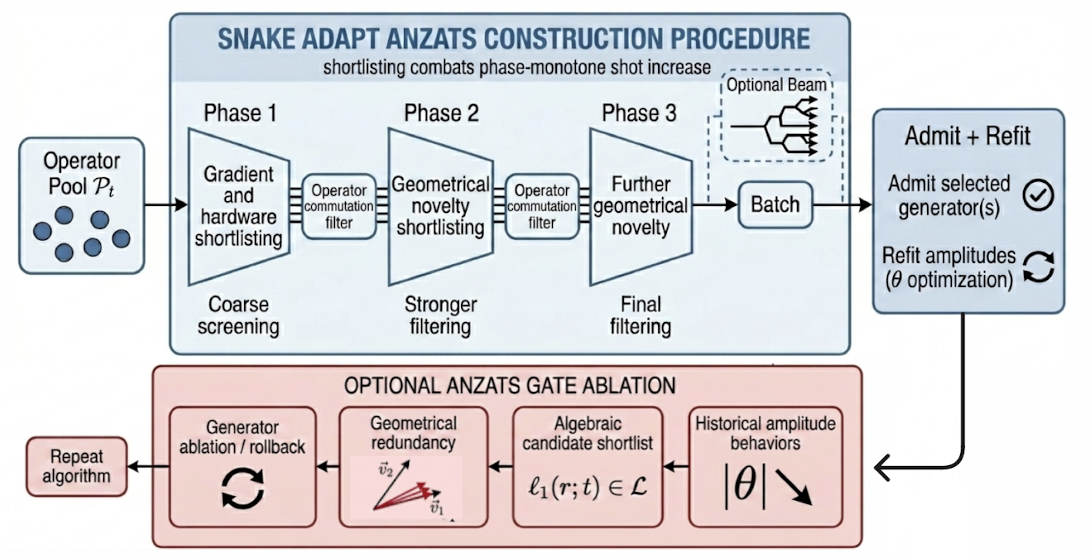
\includegraphics[width=\columnwidth]{figures/static_adapt_selector_flow_attached.png}
\captionof{figure}{SNAKE static ADAPT generator-selection flow. The broad generator pool is reduced through staged gradient--cost scoring, commutation filtering, algebraic identity shortlisting, final batch-compatible record selection, beam branching for degenerate batches, and post-admission generator-ablation.}
\label{fig:static_adapt_selector_flow}
\end{center}

\label{sec:static_method}

\subsection{Phase-zero and three-phase generator-position ranking}

SNAKE implements generator selection as a four-phase restriction of a candidate record set with entries of generator--position pairs, finalizing in top-ranked generator insertion, with conditional batching or beam branching, while a separate ablation test acts on stale entries of the existing ansatz.

Define generator set $\Gset$, and position set $\Pcal$,
\begin{equation}
\begin{aligned}
\Gset&=\{A_1,\ldots,A_m,\ldots,A_{|\Gset|}\},\\
\Pcal
&=
\left\{
p\in W(\theta;t)
\;\middle|\;
W(\theta;t)\subseteq\{1,\ldots,|U(\theta)|+1\}
\right\},
\end{aligned}
\label{eq:generator_position_sets}
\end{equation}
where $W(\theta;t)$ is a rolling window of admissible insertion positions of the existing ordered ansatz $U(\theta)$.  Define the mapping
\begin{equation}
\Phi:(\Gset,\Pcal)\longrightarrow
\mathcal R
=
\{r=(m,p)\mid A_m\in\Gset,\;p\in\Pcal\},
\label{eq:record_mapping}
\end{equation}
so $\mathcal R$ is the full candidate position-generator record set. For the staged recursion, set $\mathcal R_{-1}:=\mathcal R$, let $k\in\{0,1,2,3\}$ index the pilot or scoring phase, and let $\ell\in\mathcal L$ index the four-lane partition induced by the Cartesian product of qubit-support overlap and windowed operator-commutation status. Each stage maps $\mathcal R_{k-1}$ to $\mathcal R_k$ by lane-wise score thresholding
\begin{equation}
\mathcal R_k
:=
\bigcup_{\ell\in\mathcal L}
\left\{
r\in\mathcal R_{k-1}
\;\middle|\;
S_{k,\ell}(r)\ge\tau_{k,\ell}
\right\}.
\label{eq:phase_restriction_map}
\end{equation}
The phase score is
\begin{equation}
S_{k,\ell}(r)
=
\frac{\Delta E_k(r)\mathcal N_k(r)}{K_k(r)}.
\label{eq:master_phase_score}
\end{equation}
Here $\Delta E_k(r)$ is the phase-$k$ state-gradient gain, $\mathcal N_k(r)\in[0,1]$ is the geometric novelty factor ($\mathcal N_k(r)=1$ for $k\in\{0,1\}$), $K_k(r)$ is the hardware-cost penalty ($K_k(r)\ge1$) for record $r$, and $\tau_{k,\ell}$ is a phase- and lane-dependent threshold determined by candidate-record inter-competition. This provides the Eq.~(4)-analogous ansatz update rule,
\begin{equation}
U_{t+1}(\theta_{t+1})
=
U_t(\theta_t)
\oplus
\bigcup_{r_i\in\mathcal B\subseteq\mathcal R_3}r_i
\ominus
\bigcup_{d_j\in\mathcal D\subseteq U_t(\theta_t)}d_j .
\label{eq:snake_ansatz_update}
\end{equation}
Here $\mathcal B$ is the batch-admissible set of retained Phase-III records, and $\mathcal D$ is the ablation-admissible set of existing ansatz entries.

\subsubsection{Hardware cost penalty}

The phase-$k$ hardware-cost penalty is built from proxies estimating expected circuit burden induced from admitting candidate $r$; namely, the cost term $K$ includes: two-qubit count, layout-aware depth, one-qubit basis-change work, new parameters, and shot demand. Consider the compiled generator, $A_m=\sum_{\nu}a_{m\nu}P_{m\nu}$ where $P_{m\nu}$ is a tensor-product of Pauli matrices and identities, $\sigma \in \{I,X,Y,Z\}$. Define the Pauli-word qubit support, $S_{m\nu}:=\operatorname{supp}(P_{m\nu})=\{q:(P_{m\nu})_q\ne I\}$. Then, for a Pauli exponential compiled by a CNOT ladder, the total 2q gate count is given by,
\begin{equation}
\widehat C_{\twq}(r)=\sum_{\nu}2\,[|S_{m\nu}|-1]_+,
\label{eq:pauli_2count_proxy}
\end{equation}
whereas the layout-aware two-qubit depth is given by,
\begin{equation}
\widehat C_d(r)=\sum_{\nu}2\,\operatorname{span}_{G}
\bigl(S_{m\nu}\bigr),
\label{eq:pauli_2depth_proxy}
\end{equation}
where $G=(V,E)$ is the qubit-hardware QPU graph and $\operatorname{span}_{G}(S)$ is the number of edges in the shortest connected subgraph containing $S$, and is zero for $|S|\le1$. The same Pauli-rotation template also incurs vertex-local one-qubit basis-change work. For a local basis-change gate $\beta$, write \(c_q^{\pm}(\beta)=c_q(\beta)+c_q(\beta^{-1})\). Then
\begin{equation}
\begin{aligned}
\widehat C_{1q}(r)
=
\sum_{\nu}
\Bigg[
&\sum_{\substack{q:\\(P_{m\nu})_q=X}}
c_q^{\pm}(\beta_X)\\
&+
\sum_{\substack{q:\\(P_{m\nu})_q=Y}}
c_q^{\pm}(\beta_Y)
+
\mathbf 1_{|S_{m\nu}|>0}c_{q_{m\nu}}(R_z)
\Bigg],
\end{aligned}
\label{eq:pauli_1count_proxy}
\end{equation}
where $\beta_X$ and $\beta_Y$ are the local basis-change gates used by the Pauli-rotation template, $c_q(g)$ is the native one-qubit cost assigned to gate $g$ on vertex $q$, and $q_{m\nu}\in S_{m\nu}$ is the ladder vertex carrying the central rotation. The new-parameter feature is the increase in parameter-vector length from adding the candidate scalar coordinate $\vartheta_r$,
\begin{equation}
\widehat C_\theta(r)
=
|\theta\oplus\vartheta_r|-|\theta|.
\label{eq:parameter_cost_proxy}
\end{equation}
For measurement burden, the gradient observable underlying Eq.~(\placeholder{reference equation 3}) and Eq.~(\ref{eq:resolved_gradient}) below is partitioned into qubit-wise commuting groups $O_{r,b}=\sum_{\nu\in B_{r,b}}c_{r,b\nu}P_{r,b\nu}$. If $\mathcal B_r$ denotes this grouped Pauli partition, let $\mathcal M_t$ be the set of measurement bases already available to the selector at step $t$. For a grouped Pauli block $b\in\mathcal B_r$, write $b\preceq\mathcal M_t$ when an already cached basis measures every non-identity axis required by $b$. The cache-new groups are
\begin{equation}
\mathcal B_r^{\rm new}(t)
=
\{b\in\mathcal B_r:\,b\not\preceq\mathcal M_t\}.
\label{eq:cache_new_measurement_groups}
\end{equation}
The per-candidate shot proxy then scales as,
\begin{equation}
\widehat C_{\rm shot}(r;t)=
\frac{1}{\sigma_\star^2}
\left(
\sum_{b\in\mathcal B_r^{\rm new}(t)}
\sqrt{\sum_{\nu\in B_{r,b}}|c_{r,b\nu}|^2}
\right)^2,
\label{eq:shot_cost_proxy}
\end{equation}
where $\sigma_\star$ is the target standard error for the candidate-gradient estimate \cite{Ikhtiarudin2025ShotEfficient}. Thus candidates whose gradient observables reuse already cached measurement bases incur lower shot burden.

For a given cost term component $\widehat C_x$, the normalized excess cost is
\begin{equation}
\bar C_x(r;k):=
\operatorname{asinh}
\left(
\frac{[\widehat C_x(r)-m_x(k)]_+}{s_x(k)}
\right),
\label{eq:cost_robust_excess}
\end{equation}
where $m_x(k)$ and $s_x(k)$ are the median and robust positive scale over the live phase-$k$ record family. Measurement-grouping work supports treating Pauli burden as part of the adaptive algorithmic cost \cite{Verteletskyi2020CliqueCover,Yen2020CompatibleMeasurements}.

The phase-$k$ hardware-cost penalty then is one plus the weighted sum of these robust-normalized excess features,
\begin{equation}
\begin{aligned}
K_k(r)
={}&
1+\lambda_{\twq}\bar C_{\twq}(r;k)
+\lambda_d \bar C_d(r;k)\\
&+\lambda_{1q}\bar C_{1q}(r;k)
 +\lambda_\theta \bar C_\theta(r;k)\\
&+\lambda_{\rm shot}\bar C_{\rm shot}(r;t,k),
\end{aligned}
\label{eq:hardware_cost_sum}
\end{equation}
where each barred feature is Eq.~(\ref{eq:cost_robust_excess}) applied to its corresponding proxy. Because all terms are non-negative, $K_k(r)\ge1$.

\subsubsection{Gradient-resolution envelope}

For a candidate record $r$, SNAKE estimates the finite-resolution floor
\begin{equation}
\eta_r(t)=z_\alpha\sigma_r(t)+b_r(t),
\label{eq:gradient_resolution_floor}
\end{equation}
where $\sigma_r(t)$ is the standard error of the gradient estimate, $z_\alpha$ fixes the confidence level, and $b_r(t)$ is a backend-resolution estimate computed from hardware metrics such as compiled circuit burden, gate/readout error, coherence exposure, mitigation residuals, and calibration drift; details are given in Appendix~\ref{app:gradient_resolution_floor}. The raw ADAPT gradient and resolved gradients are,
\begin{equation}
\begin{aligned}
g_r(t)
&=
\left.
\partial_\alpha
\langle\psi_t|
e^{i\alpha\widetilde A_r}
H
e^{-i\alpha\widetilde A_r}
|\psi_t\rangle
\right|_{\alpha=0}\\
&=
i\langle\psi_t|[\widetilde A_r,H]|\psi_t\rangle,\\
\widetilde g_r(t)
&=|g_r(t)|-\eta_r(t),
\end{aligned}
\label{eq:resolved_gradient}
\end{equation}
lower bounded by zero in implementation. The Phase-I through III gain models below use this resolved gradient whenever a gradient magnitude enters a trust-region gain.

\subsubsection{Phase 0}

Phase 0 is the $k=0$ specialization of Eq.~(\ref{eq:master_phase_score}). It uses the upper-confidence first-order gradient envelope, scaled by a small pilot amplitude $\alpha_0>0$, as a pilot gain,
\begin{equation}
\Delta E_0(r;t)=\alpha_0 \left( |g_r(t)|+\eta_r(t)\right),
\label{eq:phase0_gain}
\end{equation}
so that
\begin{equation}
S_{0,\ell}(r)=\frac{\Delta E_0(r;t)}{K_0(r)}.
\label{eq:phase0_score}
\end{equation}
This removes records whose optimistic pilot energy signal is insufficient before Fubini--Study or higher-order geometric scoring.

\subsubsection{Algebraic shortlisting}

After Phase 0 assigns each candidate--position record a pilot gradient and cost score, SNAKE preserves algebraically distinct survivors before the more expensive tangent-geometry evaluation. For a live record $r=(m,p)$, let $C_1(r;t)$ denote its local candidate context, including local pool neighbors and inherited-window generators. For each $A_n\in C_1(r;t)$, define the generator-level qubit supports and the two lane predicates by
\begin{equation}
\begin{aligned}
S_m&:=\bigcup_{\nu:a_{m\nu}\ne0}S_{m\nu},
\qquad
S_n:=\bigcup_{\mu:a_{n\mu}\ne0}S_{n\mu},\\
&\operatorname{overlap}(m,n)
\Longleftrightarrow
S_m\cap S_n\ne\varnothing, \\
&\operatorname{commute}(m,n)
\Longleftrightarrow
[A_m,A_n]=0 .
\end{aligned}
\label{eq:algebraic_shortlist_checks}
\end{equation}
At the Pauli-word level, commutation is resolved by the parity of single-site anticommutations:
\begin{equation}
\begin{aligned}
&[P_{m\nu},P_{n\mu}]=0 \Longleftrightarrow \\
&\left|
\left\{
q\in S_{m\nu}\cap S_{n\mu}
:\,
(P_{m\nu})_q(P_{n\mu})_q
=-(P_{n\mu})_q(P_{m\nu})_q
\right\}
\right|\\& \equiv0\pmod 2 .
\end{aligned}
\label{eq:pauli_commutation_parity}
\end{equation}
For Pauli-expanded generators, Eq.~(\ref{eq:pauli_commutation_parity}) is applied over the nonzero Pauli-word pairs contributing to $[A_m,A_n]$; exact cancellations may be resolved by the full commutator in Eq.~(\ref{eq:algebraic_shortlist_checks}), otherwise the pair is retained in the mixed or unresolved lane. The resulting four-way shortlist preserves support-overlapping commuting records, support-overlapping noncommuting records, support-disjoint commuting records, and mixed or unresolved records. Within each lane, records remain ordered by the present phase score.

\paragraph*{Inverse Notation.}
All inverse solves below use the damped, resolved version of the displayed block. For Gram blocks, \(Q_r^+\) denotes the Moore--Penrose inverse on the resolved tangent support. We suppress explicit inverse-regularization terms in the displayed scoring equations.

\subsubsection{Phase I}

Phase I is the $k=1$ specialization of Eq.~(\ref{eq:master_phase_score}). The retained gain term $\Delta E_{1}(r)$ represents a resolution-aware energy gradient within a Fubini--Study metric trust region \cite{Nocedal2006TrustRegion}. Explicitly, for candidate $r$, let $\alpha$ denote its scalar trial amplitude,
\begin{equation}
\begin{split}
\Delta E_{1}(r)={}&\max_{|\alpha|\le \frac{\rho}{\sqrt{F_r}}} \left[\widetilde g_r(t)|\alpha|-\frac{\lambda F_r\alpha^2}{2}\right],
\end{split}
\label{eq:phase1_gain}
\end{equation}
where $\widetilde g_r(t)$ is given by Eq.~(\ref{eq:resolved_gradient}). The tangent scale is
\begin{equation}
\begin{aligned}
F_r&=\|Q_\psi\tau_r\|^2,\\
Q_\psi&=I-\ket{\psi}\bra{\psi},\\
\tau_r&=\partial_{\vartheta_r}\ket{\psi}.
\end{aligned}
\label{eq:phase1_tangent_scale}
\end{equation}
Here $\vartheta_r$ is the candidate coordinate; in implementation, a small positive floor is added to $F_r$ to prevent division by zero.
The scalar maximizer in Eq.~(\ref{eq:phase1_gain}) is explicit:
\begin{equation}
\alpha_r^\star
=
-\operatorname{sgn}\!\bigl(g_r(t)\bigr)
\min\!\left(
\dfrac{\widetilde g_r(t)}{\lambda F_r},
\dfrac{\rho}{\sqrt{F_r}}
\right).
\label{eq:phase1_alpha_star}
\end{equation}
The sign selects the descending branch of the signed gradient, while the magnitude is either the unconstrained one-dimensional quadratic optimum or the Fubini--Study trust-region boundary. If the denominator $\lambda F_r$ is zero, the quotient in Eq.~(\ref{eq:phase1_alpha_star}) is not evaluated and the magnitude is set to $\rho/\sqrt{F_r}$; after admission, the corresponding variational coordinate is optimized under the active refit policy.

\subsubsection{Phase II}

The top-ranked records from phase I are then passed into Phase II which refines the energy estimate with second-order curvature and applies a novelty bonus if the ansats-tangent window cannot express the candidates tangent. The trust-region constrained second-order energy estimate is given by,
\begin{equation}
\Delta E_{2}(r)
=\max_{|\alpha|\le \frac{ \rho}{\sqrt{F_r}}}
\Bigl[\widetilde g_r(t)|\alpha| -\frac{h_r\alpha^2}{2}\Bigr],
\label{eq:phase2_gain}
\end{equation}
where $\widetilde g_r(t)$ was defined in Eq.~(\ref{eq:resolved_gradient}). The non-negative directional curvature is,
\begin{align}
h_r&=
2\Re\!\left[
(\partial_{\alpha}\langle \psi|)H|\partial_{\alpha}\psi\rangle
+\langle\psi|H|\partial^2_{\alpha}\psi\rangle
\right],
\label{eq:phase2_hessian}\\
\partial^2_{\alpha}\ket{\psi}
&
=-(U_{>p}A_mU_{>p}^{\dagger})^2\ket{\psi}.
\label{eq:phase2_second_derivative}
\end{align}
Here \(>p\) denotes the ansats generators to the left of position index \(p\), where the right-most generator is index \(1\).

For $r$, let $i,j$ index the inherited overlap window $W_r$. The Fubini--Study Gram matrix over the refit-window and candidate-window tangent-covariance vector are given by,
\begin{equation*}
(Q_r)_{ij}=\Re\langle\tau_i,\tau_j\rangle,
\qquad
(q_r)_i=\Re\langle\tau_i,\tau_r\rangle.
\end{equation*}
The Phase-II novelty term is the normalized least-squares component of the candidate tangent lying outside the inherited-window tangent span:
\begin{equation}
\begin{aligned}
\mathcal N_2(r;t)
&:=
\frac{1}{F_r}
\min_c
\left\|
Q_\psi\left(\tau_r-\sum_{i\in W_r}c_i\tau_i\right)
\right\|^2 \\
&=
1-
\frac{q_r^{\top}Q_r^+q_r}{F_r}.
\end{aligned}
\label{eq:phase2_novelty}
\end{equation}
Thus $\mathcal N_2(r;t)$ is small when the inherited window already spans $\tau_r$, and large when the candidate contributes an independent state-space direction.

\subsubsection{Phase III}

Phase III performs a Schur-refit reranking using a . 

The Phase-III energy gain is
\begin{equation}
\Delta E_{3}(r)=
\max_{|\alpha|\le \frac{\rho}{\sqrt{F_r^\star}}}
\left[\widetilde g_r(t)|\alpha|-\frac{h_r^\star \alpha^2}{2}\right].
\label{eq:phase3_gain}
\end{equation}
Here $\widetilde g_r(t)$ is the resolved gradient from Eq.~(\ref{eq:resolved_gradient}); $F_r^\star$ and $h_r^\star$ are defined in Eqs.~(\ref{eq:phase3_star_geometry}) and~(\ref{eq:phase3_schur_response}) and represent the predicted Fubini--Study metric and the energy-curvature after admitting $r$ and allowing the existing ansats $U(\theta)$ to reoptimize.

Phase III assumes a local quadratic model of energy drop post-candidate insertion and local-window optimization. Explicitly, 
\begin{equation}
\begin{split}
E(\alpha,\delta\theta_{W_r};r)\approx{}&E_0+g_r\alpha+\frac{h_r\alpha^2}{2} \\
&+\alpha c_r^{\top}\delta\theta_{W_r}
+\frac{\delta\theta_{W_r}^{\top}H_{W_r}\delta\theta_{W_r}}{2},
\end{split}
\label{eq:local_quadratic}
\end{equation}
where $c_r$ couples the candidate to the window-response and $H_{W_r}$ is the window Hessian; entries are given by,
\begin{equation}
\begin{aligned}
(c_r)_j&:=
\left.
\frac{\partial^2E(\alpha,\delta\theta_W)}
{\partial\alpha\,\partial(\delta\theta_j)}
\right|_0,\\
(H_W)_{jk}&:=
\left.
\frac{\partial^2E(\alpha,\delta\theta_W)}
{\partial(\delta\theta_j)\,\partial(\delta\theta_k)}
\right|_0,
\qquad j,k\in W_r .
\end{aligned}
\label{eq:phase3_window_derivatives}
\end{equation}
Let \(\mathbf R_r\) denote the symmetrized inherited-window Hessian block used in the refit solve:
\begin{equation}
\mathbf R_r=\frac12(H_{W_r}+H_{W_r}^{\top}).
\label{eq:phase3_regularized_hessian}
\end{equation}
By the inverse convention above, \(\mathbf R_r^{-1}\) denotes the inverse of the damped, resolved version of this block.

Eliminating the window variables quotients out the local refit response and is given by optimizing Eq.~\ref{eq:local_quadratic} over $\delta\theta_{W_r}$ which gives the local refit displacement predicted to compensate the candidate ($\delta\theta^*_{W_r}$), which when plugged back into Eq.~(\ref{eq:local_quadratic}) yields the Schur-relaxed curvature $h^*_r$. Explicitly,
\begin{equation}
\delta\theta_W^\star=-\alpha\mathbf R_r^{-1}c_r,
\qquad
h_r^\star=h_r-c_r^{\top}\mathbf R_r^{-1}c_r .
\label{eq:phase3_schur_response}
\end{equation}
 This allows a refit-star Fubini--Study norm and refit-star candidate-window overlap:
\begin{equation}
\begin{aligned}
F_r^\star
&=F_r+2q_r^{\top}\frac{\delta\theta_W^\star}{\alpha}
+\frac{(\delta\theta_W^\star)^{\top}}{\alpha}Q_r\frac{\delta\theta_W^\star}{\alpha},\\
q_r^\star
&=q_r+Q_r\frac{\delta\theta_W^\star}{\alpha}.
\end{aligned}
\label{eq:phase3_star_geometry}
\end{equation}
Here $F_r^\star$ is the Fubini--Study norm after the inherited-window response has been optimally substituted, and $q_r^\star$ is the candidate-window overlap after the same substitution. These terms complete Eq.~(\ref{eq:phase3_gain}). A least-squares treatment analogous to Eq~(\ref{eq:phase2_novelty}) defines the Phase-III novelty factor:
\begin{equation}
\mathcal N_3(r;t)=1-\frac{(q_r^\star)^{\top}Q_r^+q_r^\star}
{F_r^\star}.
\label{eq:phase3_novelty}
\end{equation}

\subsubsection{Batching}

$B\subseteq\mathcal R_3$ is the set of eligible batch candidates that satisfy disjoint qubit support and mutually commute.

For the inherited reparameterization window associated with $B$, let $H_{BB}=[\partial_{\alpha_i}\partial_{\alpha_j}E]_{i,j=1}^s$ be the Hessian block among candidate amplitudes, and let $H_{W_BB}=[\partial_{\theta_a}\partial_{\alpha_i}E]_{a\in W_B,\,i=1,\ldots,s}$ be the mixed window-candidate block. Then, with $H_{W_BW_B}=[\partial_{\theta_a}\partial_{\theta_b}E]_{a,b\in W_B}$ and $\mathbf R_B=\frac12(H_{W_BW_B}+H_{W_BW_B}^{\top})$, the Schur-refit batch curvature is
\begin{equation}
H_B^\star
=
H_{BB}
-
H_{BW_B}\mathbf R_B^{-1}H_{W_BB}.
\label{eq:batch_schur_curvature}
\end{equation}

For an induced gradient vector of $r$, define the resolved batched gradient $\widetilde g_B(t)=\big(\widetilde g_{r_1}(t),\ldots,\widetilde g_{r_s}(t)\big)^\top$. This enables an expected batch gain,
\begin{equation}
\Delta E_3(B)
=
\max_{\alpha_B^\top G_B^\star\alpha_B\le \rho_B^2}
\left[
\widetilde g_B(t)^\top|\alpha_B|
-
\frac12\alpha_B^\top H_B^\star\alpha_B
\right],
\label{eq:batch_expected_gain}
\end{equation}
where $G_B^\star$ is the reduced Fubini--Study Gram matrix of the batch residual tangents. The admitted batch is therefore
\begin{equation}
B^\star\in\arg\max_{B\subseteq\mathcal R_3}\frac{\Delta E_3(B)}{K_3(B)}.
\label{eq:batch_argmax}
\end{equation}
In implementation, SNAKE uses greedy ordered admission rather than solving the full combinatorial batch problem.

\subsubsection{Beaming}

Under degenerate batch candidacy, SNAKE borrows Lowerre-style beam search to branch candidate circuits in parallel \cite{Lowerre1976Beam}. Each branch admits one candidate batch and undergoes the same local refit as ordinary admission. Branches are terminated once differences of energy or cost distinguish a preferred continuation.

\subsubsection{Generator ablation}

Generator ablation acts on existing ansatz entries $d_j\in U(\theta)$. For current coordinate $\theta_j$, tentative deletion is represented by the displacement $\beta_j=-\theta_j$ and an ablation refit window $W_j^\ominus$.  SNAKE reuses the Phase-III refit-window model with $\alpha$ replaced by $\beta_j$ and the candidate direction replaced by the existing coordinate being tested for deletion.  The Schur-predicted deletion loss is
\begin{equation}
\Lambda_j^\ominus
=
g_j^\ominus\beta_j
+\frac12
\left[
h_j^\ominus
-(b_j^\ominus)^{\top}(\mathbf R_j^\ominus)^{-1}b_j^\ominus
\right]\beta_j^2 .
\label{eq:ablation_schur_loss}
\end{equation}
Here $g_j^\ominus$ is the deletion-direction gradient, $h_j^\ominus$ is its directional curvature, $b_j^\ominus$ couples the deleted coordinate to $W_j^\ominus$, and $\mathbf R_j^\ominus$ is the symmetrized and damped window Hessian from Eq.~(\ref{eq:phase3_regularized_hessian}) formed on $W_j^\ominus$.  The measured post-refit deletion loss is
\begin{equation}
\Delta E_j^{\ominus,{\rm refit}}
:=
E_{\rm refit}(U_k(\theta_k)\ominus d_j)-E(U_k(\theta_k)),
\label{eq:ablation_refit_loss}
\end{equation}
and the ablation-admissible set in Eq.~(\ref{eq:snake_ansatz_update}) is
\begin{equation}
\mathcal D
=
\left\{
d_j\in U_k(\theta_k):
\begin{array}{l}
\chi_j^{\rm hist}(t)=1,\;
\Lambda_j^\ominus\le\epsilon_{\rm abl}(t),\\
\Delta E_j^{\ominus,{\rm refit}}\le\epsilon_{\rm rb}(t)
\end{array}
\right\}.
\label{eq:ablation_admissible_set}
\end{equation}
The last inequality is the rollback guard: if the accepted deletion fails after refit, the original ansatz entry is restored.

\subsection{Iteration-Dependent Gate-Selection \& Other Features}

After the staged scores in Sec.~IIA rank the live candidate records, SNAKE adapts its selection pressure using an ansatz-extension forecaster: a depth- and measurement-budgeted estimate of how many profitable insertions remain. Each accepted singleton or batch contributes a signed progress statistic given by the lower-confidence post-refit gain reduced by the marginal energy-resolution burden introduced by extending the ansatz. The forecast is built from validated ansatz improvements, signal-to-noise behavior, plateau statistics, and hardware-resolution estimates.

Early in ansatz construction, SNAKE up-biases novelty and algebraic diversity, and cost-normalized candidate penalty pressure; insertion-position windows are wider; inherited refit windows retain more coordinates; shortlist thresholds are lower; shortlist breadth is larger; and the full Phase-1/Phase-2/Phase-3 scoring sequence remains active. As the ansatz-extension forecast contracts, SNAKE downsizes insertion-position candidates, inherited refit windows, and shortlists. This contraction limits the increasing shot cost of the expanded circuit and concentrates later scoring on records whose resolved gains remain distinguishable.

The phase-local shot schedule moves in the opposite direction. Late-stage candidate gradients typically have lower signal-to-noise, so SNAKE increases phase-local shot budgets when the pilot decision signal clears the hardware-aware resolution floor. When the pilot signal falls below that floor, SNAKE spends only a diagnostic measurement budget rather than over-resolving a direction whose useful gain is not distinguishable. Expensive scoring is further limited by phase retirement: Phase 3 retires first, then Phase 2, leaving the cheaper selector as the profitable ansatz-extension forecast collapses.

The run terminates by circuit-budget saturation or by a resolved marginal-utility condition with patience: projected gradients and post-refit energy improvements must remain below the target resolvability threshold over the specified patience interval. Equivalently, no live singleton or eligible batch may retain predicted resolvable gain above the target tolerance after accounting for the marginal energy-resolution burden. Explicit formulas for the ansatz-extension forecast, feature schedules, phase retirement, shot scheduling, shortlist contraction, refit-window contraction, pruning pressure, and stopping rule are given in Appendix~\ref{app:static_ansatz_schedule_details}.

\section{Results}
\label{sec:results}
\label{sec:benchmarks}

Tables~\ref{tab:fixed_accuracy_claims}--\ref{tab:fixed_accuracy_hh_cartesian} compare SNAKE to existing ADAPT variants. We include, \texttt{Qiskit} append-only ADAPT and \texttt{Qiskit} fixed-structure VQE, using repo-native operator pools with the exception of hardware-efficient VQE. We further compare against repo-native implemented yet open-source parity checked TETRIS-ADAPT and Qubit/QEB-ADAPT, and repo-native Geo-ADAPT, and \texttt{Qiskit} fixed-structure VQE. With the exception of fixed-VQE and Qubit/QEB-ADAPT, all ADAPT variants use the same problem-local
generator pool defined in Appendix~\ref{app:pools}. Conversely, the fixed-structure VQE uses either a hardware-efficient ansats of \(R_y/R_z\) layers with nearest-neighbor CNOT entanglers, or a reasonable Hamiltonian-class motivated physical ansats, including UCCSD for fermionic systems, quadrature/HVA-style generators for bosonic
systems, and Lang-Firsov/UCCSD/quadrature hybrids for Hubbard--Holstein.  Lastly, Qubit/QEB-ADAPT is retained as a mapped-qubit excitation-pool comparator and on phonon-bearing
registers it applies qubit-excitation singles/doubles to the
binary-encoded qubits. 

For lattice and control Hamiltonians, recent Hubbard benchmark studies
report energy errors per lattice site \cite{Alvertis2024HubbardVQE},
and high-accuracy reference calculations resolve \(10^{-4}\)-scale
per-site energies in favorable regimes
\cite{LeBlanc2015HubbardBenchmarks,Qin2016AFQMCHubbard}. Following
this stricter benchmark scale, the clean \(L=2\),
unit-normalized suite uses
\[
E_T=10^{-4}LE_0=2\times10^{-4},
\]
with \(E_0=1\) set by the model unit \(t\), \(J\), or \(\omega_0\) as
appropriate.  
We then report the excess energy above this class target \(E_T=2\times 10^{-4}\), with zero indicating that the target has been reached.  Explicitly, we report
\[
\delta E=\max\!\left\{|E_{\rm alg}(n_{\rm ph}^{\rm work})-E_{\rm ref}(n_{\rm ph}^{\rm ED})|-E_T,\,0\right\}.
\]

where $E_{\rm alg}$  is the energy obtained from a VQE method, and $E_{\rm ref}$ is the energy obtained from exact-diagonalization. We use a working cutoff \(n_{\rm ph}^{\rm work}\) for VQE methods, and the reference exact-dagonalization energy uses the higher cutoff \(n_{\rm ph}^{\rm ED}\) listed in each table caption.  The working cutoff is chosen so that the ED cutoff gap \(|E_{\rm ref}(n_{\rm ph}^{\rm ED})-E_{\rm ref}(n_{\rm ph}^{\rm work})|\) is below \(E_T\).

The table fidelity diagnostic is evaluated against the exact reference state for the displayed benchmark row:
\begin{equation}
1-F=1-\left|\braket{\psi_{\rm alg}}{\psi_{\rm ref}}\right|^2 .
\label{eq:fidelity_diagnostic}
\end{equation}
Entries with \(1-F<10^{-5}\) are displayed as \(0\), so nonzero entries indicate resolved infidelity at the displayed precision.

We further compare methods in two regimes: weak and strong. For the Hubbard chain, the weak-coupling limit is controlled by
\(U/t\ll 1\), with correlation strength increasing as \(U/t\) grows;
we define \(U/t=0.5\) and \(U/t=1.5\) as the weak and strong regime, respectively
\cite{Arovas2022Hubbard}.  
For the finite-mode spin--boson/Rabi model, the conventional ultrastrong
threshold is near \(g/\omega_0\simeq 0.1\).  We therefore use
\(g/\omega_0=0.05\) as the weak point and \(g/\omega_0=0.1\) as the
stronger threshold-scale point
\cite{Kockum2019Ultrastrong,FornDiaz2019Ultrastrong}.
For Hubbard--Holstein, we follow the Holstein-dimer convention and report electron--phonon strength through \(\lambda=2g^2/(t\omega_0)\) \cite{Sakkinen2015HolsteinDimer}.  Here for
\(\omega_0/t=1\), the weak and strong Holstein benchmark sectors
\(\lambda=0.25\) and \(\lambda=1.25\) correspond to
\(g/t=\sqrt{\lambda/2}=0.354\) and \(0.791\), respectively.  The
Hubbard--Holstein benchmark uses the same weak and strong benchmark-sector convention for the Hubbard scale. We therefore report the Cartesian product of the weak and strong Hubbard vs Holstein regimes:
\((U/t,\lambda)\in\{0.25,1.25\}\times\{0.25,1.25\}\).
For further Hamiltonian instances\placeholder{list by name ones we include?} and the generators used by each, see Appendix~\ref{app:hamiltonian_families} and Appendix~\ref{app:pools} respectively. 


\begin{widetext}

% Machine provenance: native main Table I rows refreshed on 2026-05-25
% from the partial CHTC v3/v4 three-model update archive:
% tmp/chtc_partial_paper_i_three_model_v3_v4_20260525/extracted.
% Comparator rows are from cluster 6945817, and SNAKE rows are from
% cluster 6945865.
% SNAKE rows are Optuna jobs; the displayed completed SNAKE cells use the
% selected best trial in each finished job, not an arbitrary trial.
% Resource cells use Qiskit-compiled displayed-ansatz costs: first-hit ansatz
% for target hits and final terminal ansatz for non-hits.
% Fidelity cells are post-hoc reporting metrics from the same enrichment path;
% -- means the displayed source row is running, skipped, or unreconstructable.
% Support maps are regenerated by
% pipelines/reporting/build_paper_i_three_model_support_maps.py, which merges
% comparator enrichment sidecars with completed Route-A/SNAKE Optuna summaries.
% Terminal non-hit comparator costs are sourced from:
% output/pdf/paper_i_three_model_terminal_cost_recovery_20260525.json
% Hubbard depth-500 repair cells promoted from:
% output/pdf/paper_i_hubbard_depth500_repair_table_update_20260525.json
% Repair cluster 6946127 completed Pos-Geo, Qubit/QEB, append-strong, and
% TETRIS-weak rows; append-weak and TETRIS-strong were running in that snapshot.
% Running or incomplete replacement evidence must not erase prior displayed table
% data unless the user explicitly approves that destructive replacement.
% promoted sidecars:
% raw_outputs/paper_i_three_model_metric_enrichment_selected_logical_20260525_v1
% raw_outputs/paper_i_three_model_metric_enrichment_selected_logical_20260525_v2
% output/pdf/paper_i_three_model_fidelity_sources_20260525.json
% and completed CHTC v2 comparator rows fetched under:
% tmp/paper_i_three_model_comparators_v2_jsons_20260525/raw_outputs.
% Current partial update support:
% output/pdf/paper_i_three_model_partial_chtc_v3_v4_table_update_20260525.json
% output/pdf/paper_i_hubbard_table_i_prefix_fidelity_update_20260526.json
% Keep these paths in comments only; do not render them in the manuscript.

\noindent\begin{minipage}{\textwidth}
\inlinetablecaption{tab:fixed_accuracy_claims}{Hubbard fixed-accuracy current-evidence comparison at the shared target $E_T=10^{-4}LE_0=2\times10^{-4}$.  Tables~\ref{tab:fixed_accuracy_claims}--\ref{tab:fixed_accuracy_spin_boson} report target-excess error, $\delta E=\max(0,|E_{\rm alg}-E_{\rm ref}|-E_T)$, where zero indicates that the fixed target was reached.  The weak and strong columns use $U/t=0.5$ and $U/t=1.5$, respectively, where $U$ is the onsite repulsion and $t$ is the nearest-neighbor hopping.  Resource columns report Qiskit-transpiled ansatz circuits using an IBM Marrakesh backend; \(S\) is the normalized estimator/work proxy evaluated for the same ansatz.  For ADAPT methods, costs are taken at the first accepted ADAPT iteration whose energy error rounds to the displayed accuracy resolution.  Target-hit rows use the first iteration with zero target-excess error; fixed-structure VQE rows use the compiled fixed ansatz.  Fidelity columns report the corresponding post-hoc overlap diagnostic when the displayed ansatz is reconstructable.  Fidelity entries with \(1-F<10^{-5}\) are displayed as \(0\).}
% BEGIN_MACHINE_READABLE_TABLE_I_HUBBARD_SNAKE_TRUST_REGION_REPLAY_20260604
% {"schema":"paper_i_table_i_hubbard_snake_trust_region_replay_v1","updated_date":"2026-06-04","table_label":"tab:fixed_accuracy_claims","method":"SNAKE","cell":"weak","benchmark_id":"hubbard_L2_three_model_weak","source_class":"local full-meta Route-A batching-enabled Optuna diagnostic selected as cost-best target hit","selection_manifest":"tmp/paper_i_hubbard_weak_fullmeta_routeA_batching_optuna_20260604_v1/selected_cost_best_target_hit.json","selection_manifest_sha256":"db838db4de94a4599e556d5dc0dd81139cba8f0f33341a2debae3eb91ec49f5d","source_result_json":"tmp/paper_i_hubbard_weak_fullmeta_routeA_batching_optuna_20260604_v1/run/trial_0001/hubbard_L2_three_model_weak/json/result.json","source_result_sha256":"842c104bedcdd3bab209743450947bab1bae5c69a703a231f270675bc31bbc55","source_compile_json":"tmp/paper_i_hubbard_weak_fullmeta_routeA_batching_optuna_20260604_v1/run/trial_0001/hubbard_L2_three_model_weak/json/compile_scout_fake_marrakesh.json","source_compile_sha256":"d6d40502794e63539378f30632d3d5127b2600728615ec5b14c4282a711444c8","effective_trial_manifest_json":"tmp/paper_i_hubbard_weak_fullmeta_routeA_batching_optuna_20260604_v1/run/trial_0001/effective_trial_manifest.json","effective_trial_manifest_sha256":"8da40f52117fda04f9a84abd60bf5cc6bac9ccdab6bb1c6709f37a7246548cef","policy_roundtrip_audit_json":"tmp/paper_i_hubbard_weak_fullmeta_routeA_batching_optuna_20260604_v1/run/trial_0001/hubbard_L2_three_model_weak/json/policy_roundtrip_audit.json","policy_roundtrip_audit_sha256":"cb9070b2b73e9fad6b4f1e00beafd0e4f4c720d19c98670c601a2a999012aecb","exact_replay_command":"bash tmp/paper_i_hubbard_weak_fullmeta_routeA_batching_optuna_20260604_v1/run/trial_0001/hubbard_L2_three_model_weak/logs/command.sh","exact_replay_command_sha256":"c90caa53fbe8b9539d7d6e352ebaefddda6a8525e21a801ab2a26d0012306ef3","compile_replay_command":"bash tmp/paper_i_hubbard_weak_fullmeta_routeA_batching_optuna_20260604_v1/run/trial_0001/hubbard_L2_three_model_weak/logs/compile_command.sh","compile_replay_command_sha256":"7433f6ae717a4531e67533bf49c34a46c1707ffcee5f40bdc66f52f588ce3dd8","replay_note":"The replay script is the emitted adapt_pipeline CLI and writes to the original selected-trial output paths; redirect output-json/current-json to scratch before rerunning if preservation is required.","display_cell_policy":"Visible weak SNAKE target-hit and Qiskit cost cells already matched this recovered tuple; this block replaces/strengthens weak energy/cost provenance but preserves the visible table row.","display_values_supported_by_source":{"deltaE":"0","N2q":56,"D2q":52,"Dc":219},"display_values_preserved_from_existing_table_provenance":{"one_minus_F":"0","S":338},"source_values":{"k_tau":3,"energy":-1.7655479883452547,"abs_delta_e":1.6448729382112504e-05,"target_abs_delta_e":0.0002,"operators":["uccsd_dbl(ab:0,2->1,3)","uccsd_sing(beta:2->3)","uccsd_sing(alpha:0->1)"],"compiled_count_2q":56,"compiled_depth_2q":52,"compiled_depth":219,"compiled_size":256,"compiled_op_counts":{"cz":56,"rz":131,"sx":68,"x":1},"transpile_backend":"FakeMarrakesh","transpile_optimization_level":1,"transpile_seed":7},"route_settings":{"adapt_pool":"full_meta","selected_logical_route":"standard","adapt_selected_logical_mode":"off","static_route_id":"route_a","static_meta_feature_profile":"paper_i_production_v1","phase1_score_mode":"trust_region_v1","phase2_rho":0.25,"adapt_seed":7,"adapt_seed_source":"CLI default recorded in result settings","phase2_enable_batching":true,"phase3_enable_batching":true,"phase2_batch_size_cap":14,"phase2_batch_target_size":9,"phase3_batch_selection_mode":"reduced_plane","batch_selected_at_crossing":false,"adapt_reopt_policy":"windowed","adapt_window_size":29,"adapt_window_topk":87}}
% END_MACHINE_READABLE_TABLE_I_HUBBARD_SNAKE_TRUST_REGION_REPLAY_20260604
% BEGIN_MACHINE_READABLE_TABLE_I_II_VISIBLE_PREFIX_COST_AUDIT
% {"schema":"paper_i_tables_i_ii_visible_prefix_cost_audit_v1","updated_date":"2026-05-28","skill":"agent_guidance/skills/paper-i-visible-prefix-cost","spec_json":"output/pdf/paper_i_tables_i_ii_visible_prefix_cost_spec_20260528.json","audit_json":"output/pdf/paper_i_tables_i_ii_visible_prefix_cost_audit_20260528.json","criterion":"adaptive non-hit rows with adapt_history use the first accepted history prefix whose max(abs_delta_e_after-0.0002,0) renders to the displayed delta E string; fixed-structure rows are not prefix-audited","compile_helper":"pipelines.exact_bench.table_i_qiskit_resource_compile.compile_table_i_pauli_label_groups","compile_convention":"table_i_basis_gate_transpile_v1","compile_basis_gates":["id","x","sx","rx","ry","rz","h","s","sdg","cx","cz"],"transpile_optimization_level":0,"transpile_seed":7,"reference_state_rule":"auto: Hubbard HF bitstring or inferred spin-boson L=2 reference state unless source row is skipped","S_definition":"sum candidate_count_scored + selector_metric_probe_count + optimizer_nfev through selected prefix","cells":{"hubbard_append_weak":{"iter":1,"delta":"0.015","N2q":8,"D2q":4,"Dc":54,"S":185},"hubbard_tetris_weak":{"iter":0,"delta":"0.015","N2q":8,"D2q":4,"Dc":54,"S":236},"hubbard_geo_weak":{"iter":1,"delta":"0.015","N2q":8,"D2q":4,"Dc":54,"S":15064},"hubbard_qeb_weak":{"iter":1,"delta":"0.015","N2q":8,"D2q":4,"Dc":54,"S":203},"hubbard_append_strong":{"iter":1,"delta":"0.136","N2q":8,"D2q":4,"Dc":54,"S":149},"hubbard_tetris_strong":{"iter":0,"delta":"0.136","N2q":8,"D2q":4,"Dc":54,"S":39},"hubbard_qeb_strong":{"iter":1,"delta":"0.136","N2q":8,"D2q":4,"Dc":54,"S":131},"spin_boson_qeb_weak":{"iter":0,"delta":"1.47e-03","N2q":59,"D2q":59,"Dc":297,"S":11}},"skipped":{"spin_boson_qeb_strong":"source_json_missing for current nph2 strong comparator; existing resource cell preserved"}}
% END_MACHINE_READABLE_TABLE_I_II_VISIBLE_PREFIX_COST_AUDIT
% BEGIN_MACHINE_READABLE_TABLE_I_II_SPSA_OPTUNA_PROMOTION_20260601
% {"schema":"paper_i_tables_i_ii_spsa_optuna_promotion_pointer_v1","updated_date":"2026-06-01","promotion_json":"MATH/paper_facing/paper_I_static_scaffold/paper_i_tables_i_ii_spsa_optuna_current_best_promotion_20260601.json","promotion_sha256":"70c48c46288b094d1b98e373e67fb282cedb30ebbe26b5b5a524035df54e7719","source_cluster":"7096390","source_fetch_root":"raw_outputs/chtc_fetches/paper_i_table_i_ii_7096390_minimal_20260601_110736/paper_i_table_i_ii_7096390_minimal_20260601_110736","promotion_policy":"user-requested current-best SPSA Optuna comparator promotion; SNAKE rows preserved from separate SNAKE sources","fidelity_policy":"SPSA comparator artifacts do not expose exact-state fidelity, so comparator 1-F cells are displayed as --.","fixed_structure_S_policy":"fixed HEA/family SPSA rows use energy_eval_count_proxy as S; adaptive comparator rows use S_norm."}
% END_MACHINE_READABLE_TABLE_I_II_SPSA_OPTUNA_PROMOTION_20260601
\begin{center}
\footnotesize
\setlength{\tabcolsep}{1.15pt}
\renewcommand{\arraystretch}{1.08}
\begin{ruledtabular}
\begin{tabular}{p{0.145\textwidth}cccccc|cccccc}
& \multicolumn{12}{c}{Hubbard model}\\
\cline{2-13}
Method & \multicolumn{6}{c|}{Weak: $U/t=0.5$} & \multicolumn{6}{c}{Strong: $U/t=1.5$}\\
\cline{2-7}\cline{8-13}
 & \metrichead{$\delta E$} & \metrichead{$1-F$} & \metrichead{$N_{2q}$} & \metrichead{$D_{2q}$} & \metrichead{$D_c$} & \metrichead{$S$} & \metrichead{$\delta E$} & \metrichead{$1-F$} & \metrichead{$N_{2q}$} & \metrichead{$D_{2q}$} & \metrichead{$D_c$} & \metrichead{$S$}\\
\colrule
HEA VQE & 0 & -- & 6 & 5 & 35 & 4.80e4 & 0 & -- & 6 & 5 & 35 & 4.80e4\\
family VQE & 0 & -- & 56 & 52 & 278 & 4.80e4 & 0 & -- & 56 & 52 & 278 & 4.80e4\\
append ADAPT & 0.015 & -- & 56 & 52 & 274 & 1.96e4 & 0.136 & -- & 56 & 52 & 274 & 1.43e4\\
TETRIS-ADAPT & 0.016 & -- & 56 & 52 & 274 & 2.41e4 & 0.136 & -- & 56 & 52 & 274 & 2.41e4\\
Geo-ADAPT & 0 & -- & 1764 & 1699 & 8898 & 7.05e4 & 0 & -- & 376 & 364 & 1862 & 8.80e4\\
Qubit/QEB & 0.015 & -- & 56 & 52 & 274 & 4356 & 0 & -- & 56 & 52 & 274 & 2.46e4\\
SNAKE & 0 & 0 & 56 & 52 & 219 & 338 & 0 & 0 & 56 & 52 & 219 & 350\\
\end{tabular}
\end{ruledtabular}
\end{center}
\end{minipage}
\par\addvspace{1.0ex}
For the Hubbard chain, UCCSD-like structure is sufficient to hit the target, as shown by the family-informed VQE row. The HEA row is a useful caveat: despite the known tendency of hardware-efficient layers to leave conserved symmetry sectors, this small two-site instance remains accurate enough to hit the target. However, greedy first-order ADAPT selects the large-gradient singles before the double excitation; after the singles are optimized, the double is not promoted, producing a plateau. This persists for append-only ADAPT, TETRIS-ADAPT, and Qubit/QEB-ADAPT even at compiled depths above \(10^4\). Pos-Geo-ADAPT also converges in both Hubbard regimes, but we report Geo-ADAPT consistently in Tables~\ref{tab:fixed_accuracy_claims}--\ref{tab:fixed_accuracy_hh_cartesian} because the positional search incurs a runtime blow-up in the spin-boson/Rabi table and especially in the Hubbard--Holstein table. SNAKE avoids this failure through second-order Schur reranking, and therefore reaches the target in both regimes.

\noindent\begin{minipage}{\textwidth}
\inlinetablecaption{tab:fixed_accuracy_spin_boson}{Spin-boson/Rabi fixed-accuracy current-evidence comparison at the shared target $E_T=10^{-4}LE_0=2\times10^{-4}$.  The weak column uses $g/\omega_0=0.05$ with $(n_{\rm ph}^{\rm work},n_{\rm ph}^{\rm ED})=(1,5)$; the strong column uses $g/\omega_0=0.1$ with $(n_{\rm ph}^{\rm work},n_{\rm ph}^{\rm ED})=(2,6)$.  Here $g$ is the spin-mode coupling and $\omega_0$ is the mode frequency.  The error and resource columns use the same target-excess and first accepted ADAPT iteration conventions as Table~\ref{tab:fixed_accuracy_claims}.  Fidelity entries with \(1-F<10^{-5}\) are displayed as \(0\).}
% BEGIN_MACHINE_READABLE_TABLE_II_SNAKE_STRONG_SOURCE
% {"schema":"paper_i_table_ii_snake_strong_source_v1","updated_date":"2026-05-31","skill":"agent_guidance/skills/results","table_label":"tab:fixed_accuracy_spin_boson","cell":"SNAKE/strong","benchmark_id":"spin_boson_L2_nph2_three_model_strong","cutoff":{"n_ph_work":2,"n_ph_ref":6},"target_abs_delta_e":0.0002,"source_result_json":"artifacts/agent_runs/spin_boson_snake_pauli_children_no_shots_local_optuna_20260527_v1/strong/run/spin_boson_L2_nph2_three_model_strong/trial_0737/spin_boson_L2_nph2_three_model_strong/json/result.json","source_compile_json":"artifacts/agent_runs/spin_boson_snake_pauli_children_no_shots_local_optuna_20260527_v1/strong/run/spin_boson_L2_nph2_three_model_strong/trial_0737/spin_boson_L2_nph2_three_model_strong/json/compile_scout_fake_marrakesh.json","trial_number":737,"display":{"deltaE":"0","one_minus_F":"4.37e-05","N2q":174,"D2q":167,"Dc":576,"S":29},"source_values":{"primary_error_at_crossing":0.0001104134289024632,"same_cutoff_error_at_crossing":0.00011034557267213148,"one_minus_fidelity":0.000043717380653895965,"compiled_count_2q":174,"compiled_depth_2q":167,"compiled_depth":576,"controller_shot_proxy":29.0,"pool_type":"full_meta","route_id":"route_a","meta_feature_profile":"paper_i_production_v1","selected_logical_mode":"off","transpile_backend":"FakeMarrakesh"},"selection_note":"User-approved 2026-05-31 replacement of prior orphaned 170/158/575 tuple with nearest source-backed low hardware tuple from trial_0737."}
% END_MACHINE_READABLE_TABLE_II_SNAKE_STRONG_SOURCE
\begin{center}
\footnotesize
\setlength{\tabcolsep}{1.15pt}
\renewcommand{\arraystretch}{1.08}
\begin{ruledtabular}
\begin{tabular}{p{0.145\textwidth}cccccc|cccccc}
& \multicolumn{12}{c}{Spin-boson/Rabi model}\\
\cline{2-13}
Method & \multicolumn{6}{c|}{Weak: $g/\omega_0=0.05$} & \multicolumn{6}{c}{Strong: $g/\omega_0=0.1$}\\
\cline{2-7}\cline{8-13}
 & \metrichead{$\delta E$} & \metrichead{$1-F$} & \metrichead{$N_{2q}$} & \metrichead{$D_{2q}$} & \metrichead{$D_c$} & \metrichead{$S$} & \metrichead{$\delta E$} & \metrichead{$1-F$} & \metrichead{$N_{2q}$} & \metrichead{$D_{2q}$} & \metrichead{$D_c$} & \metrichead{$S$}\\
\colrule
HEA VQE & 0 & -- & 6 & 5 & 35 & 4.80e4 & 4.67e-03 & -- & 10 & 7 & 37 & 4.80e4\\
family VQE & 1.47e-03 & -- & 31 & 29 & 245 & 4.80e4 & 6.50e-03 & -- & 101 & 78 & 609 & 4.80e4\\
append ADAPT & 0 & -- & 23 & 21 & 177 & 4938 & 0 & -- & 173 & 163 & 1061 & 6269\\
TETRIS-ADAPT & 0 & -- & 23 & 21 & 177 & 4176 & 0 & -- & 173 & 163 & 1061 & 4310\\
Geo-ADAPT & 0 & -- & 23 & 21 & 177 & 5430 & 0 & -- & 593 & 583 & 4301 & 5.85e4\\
Qubit/QEB & 1.47e-03 & -- & 11 & 11 & 72 & 10 & 6.50e-03 & -- & 57 & 57 & 348 & 61\\
SNAKE & 0 & 0 & 28 & 28 & 113 & 54 & 0 & 4.37e-05 & 174 & 167 & 576 & 29\\
\end{tabular}
\end{ruledtabular}
\end{center}
\end{minipage}
\par\addvspace{1.0ex}
The spin-boson/Rabi benchmark isolates bosonic displacement and cutoff sensitivity without fermionic correlation. In the weak regime, HEA VQE and the adaptive methods reach the target, while family VQE and Qubit/QEB remain above threshold. In the strong regime, the adaptive methods and SNAKE reach the target, while HEA VQE, family VQE, and Qubit/QEB remain above threshold. Relative to the target-hit adaptive rows, SNAKE trades a higher two-qubit count and two-qubit depth for lower measurement overhead and shorter total circuit depth in both regimes.

\noindent\begin{minipage}{\textwidth}
\inlinetablecaption{tab:fixed_accuracy_hh_cartesian}{Hubbard--Holstein higher-cutoff ED-reference target-excess comparison.  Ordered pairs are $(U/t,\lambda)$, with $U$ the Hubbard onsite repulsion, $t$ the hopping, and $\lambda=2g^2/(t\omega_0)$ the Holstein coupling parameter.  The four displayed regimes are weak-weak $(0.25,0.25)$, strong-weak $(1.25,0.25)$, weak-strong $(0.25,1.25)$, and strong-strong $(1.25,1.25)$.  The Holstein-weak rows use \(n_{\rm ph}^{\rm work}=2\) and an ED5 reference, while the Holstein-strong rows use \(n_{\rm ph}^{\rm work}=4\) and an ED7 reference.  The error column reports \(\Delta E=\max\{0, |E_{\rm ref}(n_{\rm ph}^{\rm ED})-E_{\rm alg}(n_{\rm ph}^{\rm work})|-E_T\}\), where \(E_T=2\times 10^{-4}\) and \(n_{\rm ph}^{\rm ED}=n_{\rm ph}^{\rm work}+3\).  Resource columns report Qiskit-transpiled ansatz circuits using an IBM Marrakesh backend; \(S\) is the normalized estimator/work proxy evaluated for the same ansatz.  For ADAPT methods with matching accepted-history support, costs are taken at the first accepted ADAPT iteration whose \(\Delta E\) rounds to the displayed accuracy resolution.  SNAKE resource cells are preserved from their prior displayed support where matching prefix-cost provenance is not locally available.  Fidelity entries with \(1-F<10^{-5}\) are displayed as \(0\).}
% BEGIN_MACHINE_READABLE_TABLE_III_PREFIX_COST_AUDIT
% {"schema":"paper_i_table_iii_first_visible_delta_prefix_cost_v1","table_label":"tab:fixed_accuracy_hh_cartesian","updated_date":"2026-05-28","criterion":"for each adaptive non-SNAKE source JSON, choose the first adapt_history iteration whose abs_delta_e_after has the same three-significant-digit order bucket as the terminal source abs_delta_e used for the displayed Delta E; compile the cumulative selected_batch_labels prefix at that iteration","compile_helper":"pipelines.exact_bench.table_i_qiskit_resource_compile.compile_table_i_pauli_label_groups","compile_convention":"table_i_basis_gate_transpile_v1","compile_basis_gates":["id","x","sx","rx","ry","rz","h","s","sdg","cx","cz"],"transpile_optimization_level":0,"transpile_seed":7,"reference_state":"hubbard_holstein_reference_state(dims=2,n_ph_max={2 or 4},boson_encoding='binary',indexing='blocked')","pauli_group_ordering":"sorted source pool_pauli_labels_exyz for each selected label","S_firsthit_definition":"sum candidate_count_scored + selector_metric_probe_count + optimizer_nfev through the first matching iteration","snake_note":"visible SNAKE weak-Holstein cells were not recomputed because the matching same-trial JSON history or compiled sidecar for the displayed 7.41e-4/3.45e-4 cells was not found locally","cells":{"append_ww":{"iter":3,"delta_iter":0.001495733258212284,"N2q":96,"D2q":68,"Dc":503,"S":483},"append_sw":{"iter":3,"delta_iter":0.07813825286766879,"N2q":96,"D2q":68,"Dc":503,"S":917},"append_ws":{"iter":7,"delta_iter":0.04763766364527733,"N2q":760,"D2q":636,"Dc":3563,"S":3556},"append_ss":{"iter":11,"delta_iter":0.0329493488257806,"N2q":1240,"D2q":876,"Dc":4911,"S":7619},"tetris_ww":{"iter":2,"delta_iter":0.001495733258212617,"N2q":96,"D2q":68,"Dc":503,"S":646},"tetris_sw":{"iter":2,"delta_iter":0.07813825286766946,"N2q":96,"D2q":68,"Dc":503,"S":478},"tetris_ws":{"iter":5,"delta_iter":0.04763757844699601,"N2q":1240,"D2q":629,"Dc":3665,"S":3002},"tetris_ss":{"iter":8,"delta_iter":0.03294774390507804,"N2q":2080,"D2q":1098,"Dc":6364,"S":10291},"geo_ww":{"iter":322,"delta_iter":0.0007134974956946039,"N2q":15816,"D2q":15581,"Dc":81541,"S":587371},"geo_sw":{"iter":83,"delta_iter":0.00033536944035472693,"N2q":4084,"D2q":3999,"Dc":22592,"S":161273},"geo_ws":{"iter":342,"delta_iter":0.047649993779623756,"N2q":35008,"D2q":33853,"Dc":182574,"S":760776},"geo_ss":{"iter":207,"delta_iter":0.013048857559364024,"N2q":17680,"D2q":17265,"Dc":91487,"S":460503},"qeb_ww":{"iter":1,"delta_iter":0.04335311949924381,"N2q":8,"D2q":4,"Dc":54,"S":655},"qeb_sw":{"iter":1,"delta_iter":0.11999563910870042,"N2q":8,"D2q":4,"Dc":54,"S":650},"qeb_ws":{"iter":1,"delta_iter":0.2635792003593468,"N2q":8,"D2q":4,"Dc":54,"S":1394},"qeb_ss":{"iter":1,"delta_iter":0.24891040483138988,"N2q":8,"D2q":4,"Dc":54,"S":1422}}}
% END_MACHINE_READABLE_TABLE_III_PREFIX_COST_AUDIT
% BEGIN_MACHINE_READABLE_TABLE_III_HH_WEAK_HOLSTEIN_UPDATE_20260530
% {
%   "schema": "paper_i_table_iii_hh_weak_holstein_update_sources_v2",
%   "table_label": "tab:fixed_accuracy_hh_cartesian",
%   "updated_date": "2026-05-30",
%   "updated_columns": ["weak_weak", "strong_weak"],
%   "target_abs_delta_e": 0.0002,
%   "display_delta_e_policy": "max(0, abs(E_alg(n_ph_work)-E_exact(n_ph_ref)) - target_abs_delta_e)",
%   "cutoff_contract": {
%     "weak_weak": {"n_ph_work": 2, "n_ph_ref": 5},
%     "strong_weak": {"n_ph_work": 2, "n_ph_ref": 5}
%   },
%   "source_roots": {
%     "fixed_and_qeb_update_20260527": "output/pdf/paper_i_hh_symmetric_table_iii_partial_update_20260527.json",
%     "comparators_newpool": "raw_outputs/chtc_fetches/hh_tableiii_status_minimal_20260530_095918/raw_outputs/paper_i_hh_symmetric_comparators_full_meta_newpool_20260530_v1",
%     "snake_weak_weak": "output/pdf/paper_i_table_iii_snake_weak_weak_live_prefix_promotion_20260530.json",
%     "snake_strong_weak": "raw_outputs/chtc_fetches/hh_snake_live_snapshot_20260530_113725/7016920.1.txt"
%   },
%   "warnings": [
%     "Comparator full-meta-newpool artifacts expose same-cutoff exact errors but do not embed the ED5 external-reference energy; the cutoff floor recorded here is inferred from the matching SNAKE external-reference diagnostic.",
%     "This overlay supersedes weak-Holstein Delta E cells in the older prefix-cost audit; that older audit remains historical prefix-cost provenance.",
%     "SNAKE weak-weak is promoted from a live running CHTC checkpoint by explicit user request; the underlying Optuna job remains running.",
%     "SNAKE strong-weak is sourced from a live current_best snapshot, not a final CHTC summary."
%   ],
%   "cells": {
%     "hea_ww": {
%       "method": "HEA VQE",
%       "regime": "weak_weak",
%       "source_root": "fixed_and_qeb_update_20260527",
%       "source_record": "visible_table_rows:static_table__hh__hh_L2_nph2_three_model_sym_weak_weak__static_hea_qiskit_vqe",
%       "evidence_status": "completed_summary",
%       "raw_external_abs_delta_e": 0.021414764555328203,
%       "display_delta_e_source": "external_abs_delta_e_minus_target",
%       "display_delta_e": 0.021214764555328204,
%       "visible_cells": {"DeltaE": "0.0212", "one_minus_F": "--", "N2q": 56, "D2q": 21, "Dc": 111, "S": 8000}
%     },
%     "family_ww": {
%       "method": "family VQE",
%       "regime": "weak_weak",
%       "source_root": "fixed_and_qeb_update_20260527",
%       "source_record": "visible_table_rows:static_table__hh__hh_L2_nph2_three_model_sym_weak_weak__static_family_informed_vqe",
%       "evidence_status": "completed_summary",
%       "raw_external_abs_delta_e": 0.8587572024680334,
%       "display_delta_e_source": "external_abs_delta_e_minus_target",
%       "display_delta_e": 0.8585572024680335,
%       "visible_cells": {"DeltaE": "0.8586", "one_minus_F": "--", "N2q": 1394, "D2q": 1166, "Dc": 5863, "S": 1065}
%     },
%     "qeb_ww": {
%       "method": "Qubit/QEB",
%       "regime": "weak_weak",
%       "source_root": "fixed_and_qeb_update_20260527",
%       "source_record": "visible_table_rows:static_table__hh__hh_L2_nph2_three_model_sym_weak_weak__static_qubit_qeb_adapt_vqe",
%       "evidence_status": "completed_summary",
%       "pool_contract": "qeb",
%       "raw_external_abs_delta_e": 0.04338146473683313,
%       "display_delta_e_source": "external_abs_delta_e_minus_target",
%       "display_delta_e": 0.04318146473683313,
%       "visible_cells": {"DeltaE": "0.0432", "one_minus_F": "--", "N2q": 8, "D2q": 4, "Dc": 54, "S": 655}
%     },
%     "append_ww": {
%       "method": "append ADAPT",
%       "regime": "weak_weak",
%       "source_root": "comparators_newpool",
%       "source_record": "static_table__hh__hh_L2_nph2_three_model_sym_weak_weak__static_full_meta_append_adapt_vqe/result/generic_static_single.json",
%       "source_cluster": "6996346.1",
%       "evidence_status": "completed_summary",
%       "pool_contract": "full_meta",
%       "raw_same_cutoff_abs_delta_e": 0.0005729997306191947,
%       "cutoff_floor_from_snake_reference": 0.000028345237591542727,
%       "raw_external_abs_delta_e_inferred": 0.0006013449682107374,
%       "display_delta_e_source": "external_abs_delta_e_inferred_minus_target",
%       "display_delta_e": 0.00040134496821073743,
%       "visible_cells": {"DeltaE": "4.01e-4", "one_minus_F": "--", "N2q": 1002, "D2q": 874, "Dc": 4048, "S": 11988}
%     },
%     "tetris_ww": {
%       "method": "TETRIS-ADAPT",
%       "regime": "weak_weak",
%       "source_root": "comparators_newpool",
%       "source_record": "static_table__hh__hh_L2_nph2_three_model_sym_weak_weak__static_tetris_qubit_adapt_vqe/result/generic_static_single.json",
%       "source_cluster": "6996346.4",
%       "evidence_status": "completed_summary",
%       "pool_contract": "full_meta",
%       "raw_same_cutoff_abs_delta_e": 0.0011270037450819004,
%       "cutoff_floor_from_snake_reference": 0.000028345237591542727,
%       "raw_external_abs_delta_e_inferred": 0.001155348982673443,
%       "display_delta_e_source": "external_abs_delta_e_inferred_minus_target",
%       "display_delta_e": 0.000955348982673443,
%       "visible_cells": {"DeltaE": "9.55e-4", "one_minus_F": "--", "N2q": 460, "D2q": 385, "Dc": 1721, "S": 4549}
%     },
%     "geo_ww": {
%       "method": "Geo-ADAPT",
%       "regime": "weak_weak",
%       "source_root": "comparators_newpool",
%       "source_record": "static_table__hh__hh_L2_nph2_three_model_sym_weak_weak__static_geo_adapt_vqe/result/generic_static_single.json",
%       "source_cluster": "6996346.7",
%       "evidence_status": "completed_summary",
%       "pool_contract": "full_meta",
%       "raw_same_cutoff_abs_delta_e": 0.0011283369617475225,
%       "cutoff_floor_from_snake_reference": 0.000028345237591542727,
%       "raw_external_abs_delta_e_inferred": 0.0011566821993390652,
%       "display_delta_e_source": "external_abs_delta_e_inferred_minus_target",
%       "display_delta_e": 0.0009566821993390653,
%       "visible_cells": {"DeltaE": "9.57e-4", "one_minus_F": "--", "N2q": 4482, "D2q": 2587, "Dc": 40952, "S": 2579686}
%     },
%     "snake_ww": {
%       "method": "SNAKE",
%       "regime": "weak_weak",
%       "source_root": "snake_weak_weak",
%       "source_record": "paper_i_table_iii_snake_weak_weak_live_prefix_promotion_20260530.json",
%       "evidence_status": "live_running_checkpoint_not_trial_final",
%       "pool_contract": "New Full Meta",
%       "best_trial": 0,
%       "chosen_prefix_policy": "first accepted prefix whose displayed DeltaE matches the live current-best DeltaE within 5e-9",
%       "chosen_prefix_len": 11,
%       "chosen_depth": 11,
%       "energy_adapt_n_ph_work": -0.9179301830083294,
%       "energy_exact_reference_cutoff": -0.9183814647368329,
%       "raw_external_abs_delta_e": 0.00045128172850350534,
%       "display_delta_e_source": "external_abs_delta_e_minus_target",
%       "display_delta_e": 0.00025128172850350536,
%       "compile_convention": "table_i_basis_gate_transpile_v1",
%       "S_norm_status": "native_controller_work_live_prefix_proxy",
%       "visible_cells": {"DeltaE": "2.51e-4", "one_minus_F": "--", "N2q": 124, "D2q": 48, "Dc": 773, "S": 3658}
%     },
%     "hea_sw": {
%       "method": "HEA VQE",
%       "regime": "strong_weak",
%       "source_root": "fixed_and_qeb_update_20260527",
%       "source_record": "visible_table_rows:static_table__hh__hh_L2_nph2_three_model_sym_strong_weak__static_hea_qiskit_vqe",
%       "evidence_status": "completed_summary",
%       "raw_external_abs_delta_e": 0.020551289729370814,
%       "display_delta_e_source": "external_abs_delta_e_minus_target",
%       "display_delta_e": 0.020351289729370815,
%       "visible_cells": {"DeltaE": "0.0204", "one_minus_F": "--", "N2q": 56, "D2q": 21, "Dc": 111, "S": 8000}
%     },
%     "family_sw": {
%       "method": "family VQE",
%       "regime": "strong_weak",
%       "source_root": "fixed_and_qeb_update_20260527",
%       "source_record": "visible_table_rows:static_table__hh__hh_L2_nph2_three_model_sym_strong_weak__static_family_informed_vqe",
%       "evidence_status": "completed_summary",
%       "raw_external_abs_delta_e": 0.8052069398468328,
%       "display_delta_e_source": "external_abs_delta_e_minus_target",
%       "display_delta_e": 0.8050069398468328,
%       "visible_cells": {"DeltaE": "0.8050", "one_minus_F": "--", "N2q": 1394, "D2q": 1166, "Dc": 5863, "S": 1299}
%     },
%     "qeb_sw": {
%       "method": "Qubit/QEB",
%       "regime": "strong_weak",
%       "source_root": "fixed_and_qeb_update_20260527",
%       "source_record": "visible_table_rows:static_table__hh__hh_L2_nph2_three_model_sym_strong_weak__static_qubit_qeb_adapt_vqe",
%       "evidence_status": "completed_summary",
%       "pool_contract": "qeb",
%       "raw_external_abs_delta_e": 0.12000550257876219,
%       "display_delta_e_source": "external_abs_delta_e_minus_target",
%       "display_delta_e": 0.11980550257876219,
%       "visible_cells": {"DeltaE": "0.1198", "one_minus_F": "--", "N2q": 8, "D2q": 4, "Dc": 54, "S": 650}
%     },
%     "append_sw": {
%       "method": "append ADAPT",
%       "regime": "strong_weak",
%       "source_root": "comparators_newpool",
%       "source_record": "static_table__hh__hh_L2_nph2_three_model_sym_strong_weak__static_full_meta_append_adapt_vqe/result/generic_static_single.json",
%       "source_cluster": "6996346.2",
%       "evidence_status": "completed_summary",
%       "pool_contract": "full_meta",
%       "raw_same_cutoff_abs_delta_e": 0.026807853728359754,
%       "cutoff_floor_from_snake_reference": 0.000009863470061988178,
%       "raw_external_abs_delta_e_inferred": 0.026817717198421742,
%       "display_delta_e_source": "external_abs_delta_e_inferred_minus_target",
%       "display_delta_e": 0.026617717198421743,
%       "visible_cells": {"DeltaE": "0.0266", "one_minus_F": "--", "N2q": 2362, "D2q": 2061, "Dc": 9922, "S": 179389}
%     },
%     "tetris_sw": {
%       "method": "TETRIS-ADAPT",
%       "regime": "strong_weak",
%       "source_root": "comparators_newpool",
%       "source_record": "static_table__hh__hh_L2_nph2_three_model_sym_strong_weak__static_tetris_qubit_adapt_vqe/result/generic_static_single.json",
%       "source_cluster": "6996346.5",
%       "evidence_status": "completed_summary",
%       "pool_contract": "full_meta",
%       "raw_same_cutoff_abs_delta_e": 0.077769523341427,
%       "cutoff_floor_from_snake_reference": 0.000009863470061988178,
%       "raw_external_abs_delta_e_inferred": 0.07777938681148899,
%       "display_delta_e_source": "external_abs_delta_e_inferred_minus_target",
%       "display_delta_e": 0.07757938681148899,
%       "visible_cells": {"DeltaE": "0.0776", "one_minus_F": "--", "N2q": 172, "D2q": 98, "Dc": 750, "S": 2326}
%     },
%     "geo_sw": {
%       "method": "Geo-ADAPT",
%       "regime": "strong_weak",
%       "source_root": "comparators_newpool",
%       "source_record": "static_table__hh__hh_L2_nph2_three_model_sym_strong_weak__static_geo_adapt_vqe/result/generic_static_single.json",
%       "source_cluster": "6996346.8",
%       "evidence_status": "completed_summary",
%       "pool_contract": "full_meta",
%       "raw_same_cutoff_abs_delta_e": 0.00017578634511455915,
%       "cutoff_floor_from_snake_reference": 0.000009863470061988178,
%       "raw_external_abs_delta_e_inferred": 0.00018564981517654733,
%       "display_delta_e_source": "max(0, external_abs_delta_e_inferred_minus_target)",
%       "display_delta_e": 0,
%       "visible_cells": {"DeltaE": "0", "one_minus_F": "--", "N2q": 10610, "D2q": 9204, "Dc": 73153, "S": 2116564}
%     },
%     "snake_sw": {
%       "method": "SNAKE",
%       "regime": "strong_weak",
%       "source_root": "snake_strong_weak",
%       "source_record": "7016920.1.txt current_best payload",
%       "evidence_status": "live_snapshot_not_final_summary",
%       "pool_contract": "full_meta",
%       "best_trial": 11,
%       "best_value": 20.131755854051008,
%       "energy_adapt_n_ph_work": -0.4948179071703059,
%       "energy_exact_reference_cutoff": -0.49500550257876286,
%       "raw_external_abs_delta_e": 0.0001875954084569753,
%       "raw_same_cutoff_abs_delta_e": 0.00017773193839498713,
%       "cutoff_floor": 0.000009863470061988178,
%       "display_delta_e_source": "max(0, external_abs_delta_e_minus_target)",
%       "display_delta_e": 0,
%       "objective_weights": {"energy": 32.0, "count_2q": 0.0, "depth_2q": 0.0, "circuit_depth": 0.0, "parameters": 0.0, "shot_cost": 0.0},
%       "visible_cells": {"DeltaE": "0", "one_minus_F": "--", "N2q": 314, "D2q": 243, "Dc": 801, "S": 7549}
%     }
%   }
% }
% END_MACHINE_READABLE_TABLE_III_HH_WEAK_HOLSTEIN_UPDATE_20260530
%
% BEGIN_MACHINE_READABLE_TABLE_III_HH_STRONG_HOLSTEIN_COMPLETION_20260530
% {
%   "schema": "paper_i_table_iii_hh_strong_holstein_completion_sources_v1",
%   "table_label": "tab:fixed_accuracy_hh_cartesian",
%   "updated_date": "2026-05-30",
%   "updated_columns": [
%     "weak_strong",
%     "strong_strong"
%   ],
%   "target_abs_delta_e": 0.0002,
%   "display_delta_e_policy": "max(0, abs(E_alg(n_ph_work)-E_exact(n_ph_ref)) - target_abs_delta_e)",
%   "cutoff_contract": {
%     "weak_strong": {
%       "n_ph_work": 4,
%       "n_ph_ref": 7
%     },
%     "strong_strong": {
%       "n_ph_work": 4,
%       "n_ph_ref": 7
%     }
%   },
%   "source_roots": {
%     "new_full_meta_newpool": "raw_outputs/chtc_fetches/hh_tableiii_status_minimal_20260530_095918/raw_outputs/paper_i_hh_symmetric_comparators_full_meta_newpool_20260530_v1",
%     "older_completed_full_meta_provenance": "output/pdf/paper_i_hh_table3_adapt_descent_all_regimes_prefix23_logy.provenance.json",
%     "snake_weak_strong_checkpoint": "output/pdf/paper_i_table_iii_snake_weak_strong_stopped_checkpoint_qiskit_cost_20260529.json",
%     "snake_strong_strong_checkpoint": "output/pdf/paper_i_table_iii_snake_checkpoint_qiskit_costs_20260529.json",
%     "snake_all_time_best_weak_strong_result": "raw_outputs/chtc_fetches/hh_snake_all_time_best_ws_ss_20260531/hh_ws_trial0004_result.json",
%     "snake_all_time_best_weak_strong_cost": "output/pdf/paper_i_table_iii_snake_weak_strong_costpreserve_trial0004_qiskit_cost_20260531.json",
%     "snake_all_time_best_strong_strong_result": "raw_outputs/chtc_fetches/hh_snake_all_time_best_ws_ss_20260531/hh_ss_trial0001_result.json",
%     "snake_all_time_best_strong_strong_cost": "output/pdf/paper_i_table_iii_snake_strong_strong_costpreserve_trial0001_qiskit_cost_20260531.json",
%     "snake_current_best_provenance_txt": "MATH/paper_facing/paper_I_static_scaffold/hh_tableiii_snake_current_best_provenance_20260531.txt"
%   },
%   "cells": {
%     "weak_strong": {
%       "append ADAPT": {
%         "display_delta_e": 0.0476,
%         "resource_tuple": [760, 636, 3563, 3556],
%         "source_policy": "preserved older completed full-meta result; targeted cleanup rerun queued"
%       },
%       "TETRIS-ADAPT": {
%         "display_delta_e": 0.0476,
%         "resource_tuple": [1240, 629, 3665, 3002],
%         "source_policy": "preserved older completed full-meta result; targeted cleanup rerun queued"
%       },
%       "Geo-ADAPT": {
%         "display_delta_e": 0.0302,
%         "raw_abs_delta_e_external_ref": 0.030394553865939145,
%         "cutoff_floor_abs_delta_e": 0.00014143771565588992,
%         "resource_tuple": [109756, 103316, 609633, 2706229],
%         "source_record_id": "static_table__hh__hh_L2_nph4_three_model_sym_weak_strong__static_geo_adapt_vqe",
%         "source_policy": "new completed full-meta-newpool result"
%       },
%       "SNAKE": {
%         "display_delta_e": 0.0376,
%         "raw_abs_delta_e_external_ref": 0.037753313683037915,
%         "resource_tuple": [1592, 1282, 7194, null],
%         "source_result_sha256": "617a55bcafbbc97a95103263fd40edff1c60163ba04b52514ff45a2788765313",
%         "compiled_cost_sha256": "b63650c97fda3eef11aa1778cddda689f39fb4b7e67b0ca59e342654a2d36170",
%         "source_policy": "completed CHTC cost-preserve trial_0004 all-time best so far; full S_norm unavailable"
%       }
%     },
%     "strong_strong": {
%       "append ADAPT": {
%         "display_delta_e": 0.00389,
%         "raw_abs_delta_e_external_ref": 0.004093570030601512,
%         "cutoff_floor_abs_delta_e": 0.00002920892050450874,
%         "resource_tuple": [28724, 26701, 99051, 578256],
%         "source_record_id": "static_table__hh__hh_L2_nph4_three_model_sym_strong_strong__static_full_meta_append_adapt_vqe",
%         "source_policy": "new completed full-meta-newpool result"
%       },
%       "TETRIS-ADAPT": {
%         "display_delta_e": 0.0329,
%         "resource_tuple": [2080, 1098, 6364, 10291],
%         "source_policy": "preserved older completed full-meta result; targeted cleanup rerun queued"
%       },
%       "Geo-ADAPT": {
%         "display_delta_e": 0.0130,
%         "resource_tuple": [17680, 17265, 91487, 461000],
%         "source_policy": "preserved older completed full-meta result because new completed full-meta-newpool result was worse"
%       },
%       "SNAKE": {
%         "display_delta_e": 0.00867,
%         "raw_abs_delta_e_external_ref": 0.008872910477360385,
%         "resource_tuple": [956, 918, 5350, null],
%         "source_result_sha256": "e10ff56167e76c2e8c173c46a5e4a93d0fe966e5638f58945afa5c52de322b12",
%         "compiled_cost_sha256": "6e72c296cbb6d667459645f89704c6e3484d5e9030a0f48ed32c4f9c999b2a56",
%         "source_policy": "completed CHTC cost-preserve trial_0001 all-time best so far; full S_norm unavailable"
%       }
%     }
%   },
%   "residual_chtc_cleanup": {
%     "reason": "new full-meta-newpool CHTC fetch did not contain completed result JSON for three rows; visible cells preserve older completed full-meta evidence while targeted cleanup rows rerun",
%     "records": [
%       {
%         "regime": "weak_strong",
%         "method": "append ADAPT",
%         "record_id": "static_table__hh__hh_L2_nph4_three_model_sym_weak_strong__static_full_meta_append_adapt_vqe",
%         "previous_proc": "6996346.3"
%       },
%       {
%         "regime": "weak_strong",
%         "method": "TETRIS-ADAPT",
%         "record_id": "static_table__hh__hh_L2_nph4_three_model_sym_weak_strong__static_tetris_qubit_adapt_vqe",
%         "previous_proc": "6996346.11"
%       },
%       {
%         "regime": "strong_strong",
%         "method": "TETRIS-ADAPT",
%         "record_id": "static_table__hh__hh_L2_nph4_three_model_sym_strong_strong__static_tetris_qubit_adapt_vqe",
%         "previous_proc": "6996346.10"
%       }
%     ]
%   }
% }
% END_MACHINE_READABLE_TABLE_III_HH_STRONG_HOLSTEIN_COMPLETION_20260530
% BEGIN_MACHINE_READABLE_TABLE_III_HH_SNAKE_STDOUT_CONTINUATION_PROMOTION_20260601
% {"schema":"paper_i_table_iii_hh_snake_stdout_continuation_promotion_pointer_v1","updated_date":"2026-06-01","promotion_json":"MATH/paper_facing/paper_I_static_scaffold/paper_i_table_iii_hh_snake_stdout_continuation_promotion_20260601.json","promotion_sha256":"292336b54ffc577c72690646815634b6986e3323557f795cfe5c262f6f766bbf","source_map":"MATH/paper_facing/paper_I_static_scaffold/hh_tableiii_convergence_sources.json","visible_table_changes":[{"regime":"weak_strong","method":"SNAKE","field":"DeltaE","new_value":"0.0184","raw_external_abs_delta_e":0.018593762719976814},{"regime":"strong_strong","method":"SNAKE","field":"DeltaE","new_value":"0.00767","raw_external_abs_delta_e":0.007870712035234706}],"resource_cell_policy":"SNAKE weak-strong and strong-strong resource cells are retained from prior JSON-backed compiled-cost sidecars because the running continuation jobs exposed stdout AI_LOG progress but no replayable current/result JSON at promotion time.","status":"visible Table III SNAKE weak-strong and strong-strong DeltaE cells promoted from fetched live stdout continuation; strict replay remains blocked until continuation JSON is recovered."}
% END_MACHINE_READABLE_TABLE_III_HH_SNAKE_STDOUT_CONTINUATION_PROMOTION_20260601
% BEGIN_MACHINE_READABLE_TABLE_III_HH_SPSA_OPTUNA_PROMOTION_20260601
% {"schema":"paper_i_table_iii_hh_spsa_optuna_promotion_pointer_v1","updated_date":"2026-06-01","promotion_json":"MATH/paper_facing/paper_I_static_scaffold/paper_i_table_iii_hh_spsa_optuna_current_best_promotion_20260601.json","promotion_sha256":"f5b0127b64340973cfd793ed60b9f9fec0f712d66eb4affd344e06286bddf3fd","geo_incomplete_note":"MATH/paper_facing/paper_I_static_scaffold/paper_i_table_iii_hh_geo_spsa_incomplete_note_20260601.txt","geo_incomplete_note_sha256":"13f6d0033a3f032ae940d4116e3451d9860d27efb4dee94ababc38454aaeabd7","source_cluster":"7096390","source_fetch_root":"raw_outputs/chtc_fetches/paper_i_hh_tableiii_spsa_7096390_minimal_20260601/paper_i_hh_tableiii_spsa_minimal_20260601_120550","promotion_policy":"promote usable SPSA Optuna current-best comparator rows; preserve Geo-ADAPT because SPSA calibration is incomplete; preserve Qubit/QEB weak-strong and strong-strong because SPSA completed with zero usable trials; preserve SNAKE from separate SNAKE sources.","fidelity_policy":"SPSA comparator artifacts do not expose exact-state fidelity, so affected comparator 1-F cells are displayed as --.","fixed_structure_S_policy":"HEA/family SPSA rows use energy_eval_count_proxy as S; adaptive comparator rows use S_norm."}
% END_MACHINE_READABLE_TABLE_III_HH_SPSA_OPTUNA_PROMOTION_20260601
% BEGIN_MACHINE_READABLE_TABLE_III_HH_GEO_QEB_SPSA_REPAIR_PROMOTION_20260604
% {"schema":"paper_i_table_iii_hh_geo_qeb_spsa_repair_promotion_pointer_v1","updated_date":"2026-06-04","promotion_json":"MATH/paper_facing/paper_I_static_scaffold/paper_i_table_iii_hh_geo_qeb_spsa_repair_promotion_20260604.json","promotion_sha256":"72a749152c1600f9a91e548ba96c7ecdc77637abf7b56b6beb7add9fb1b1b6bb","source_cluster":"7408967","source_fetch_root":"raw_outputs/chtc_fetches/hh_geo_qeb_spsa_repair_v1_7408967","source_archive_sha256":"0d791fcc8ce92f75b3016643d6946764984da0cdf6ed97130aa83c369a0d40a4","visible_table_changes":["Geo-ADAPT all four regimes replaced by completed SPSA repair current bests","Qubit/QEB all four regimes replaced by completed SPSA repair current bests"],"promotion_policy":"completed Geo-ADAPT and Qubit/QEB SPSA repair replaces previously preserved/incomplete Geo/QEB cells; HEA, family VQE, append ADAPT, TETRIS-ADAPT, and SNAKE are preserved from existing SPSA/SNAKE source maps, so every visible Table III algorithm is SPSA-backed."}
% END_MACHINE_READABLE_TABLE_III_HH_GEO_QEB_SPSA_REPAIR_PROMOTION_20260604
\begin{center}
\footnotesize
\setlength{\tabcolsep}{1.15pt}
\renewcommand{\arraystretch}{1.08}
\begin{ruledtabular}
\begin{tabular}{p{0.145\textwidth}cccccc|cccccc}
& \multicolumn{12}{c}{Hubbard-Holstein model, Holstein weak: $\lambda=0.25$}\\
\cline{2-13}
Method & \multicolumn{6}{c|}{Weak-weak: $(U/t,\lambda)=(0.25,0.25)$} & \multicolumn{6}{c}{Strong-weak: $(U/t,\lambda)=(1.25,0.25)$}\\
\cline{2-7}\cline{8-13}
 & \metrichead{$\Delta E$} & \metrichead{$1-F$} & \metrichead{$N_{2q}$} & \metrichead{$D_{2q}$} & \metrichead{$D_c$} & \metrichead{$S$} & \metrichead{$\Delta E$} & \metrichead{$1-F$} & \metrichead{$N_{2q}$} & \metrichead{$D_{2q}$} & \metrichead{$D_c$} & \metrichead{$S$}\\
\colrule
HEA VQE & 0.0337 & -- & 14 & 9 & 39 & 4.80e4 & 0.0244 & -- & 14 & 9 & 39 & 4.80e4\\
family VQE & 0.9778 & -- & 1782 & 1614 & 7003 & 4.80e4 & 0.9183 & -- & 1782 & 1614 & 7003 & 4.80e4\\
append ADAPT & 9.59e-4 & -- & 4384 & 4131 & 15624 & 3.13e4 & 0.0776 & -- & 4288 & 4058 & 15352 & 5.95e4\\
TETRIS-ADAPT & 9.56e-4 & -- & 4384 & 4040 & 14931 & 5.43e4 & 0.0776 & -- & 4384 & 4047 & 14960 & 3.18e4\\
Geo-ADAPT & 9.56e-4 & -- & 278 & 159 & 2053 & 2.03e5 & 0 & -- & 292 & 286 & 1569 & 6.74e4\\
Qubit/QEB & 0.0431 & -- & 1044 & 1021 & 4932 & 7.37e4 & 0.0244 & -- & 1696 & 1656 & 8007 & 1.11e5\\
SNAKE & 2.51e-4 & -- & 124 & 48 & 773 & 3658 & 0 & -- & 314 & 243 & 801 & 7549\\
\colrule
& \multicolumn{12}{c}{Hubbard-Holstein model, Holstein strong: $\lambda=1.25$}\\
\cline{2-13}
Method & \multicolumn{6}{c|}{Weak-strong: $(U/t,\lambda)=(0.25,1.25)$} & \multicolumn{6}{c}{Strong-strong: $(U/t,\lambda)=(1.25,1.25)$}\\
\cline{2-7}\cline{8-13}
 & \metrichead{$\Delta E$} & \metrichead{$1-F$} & \metrichead{$N_{2q}$} & \metrichead{$D_{2q}$} & \metrichead{$D_c$} & \metrichead{$S$} & \metrichead{$\Delta E$} & \metrichead{$1-F$} & \metrichead{$N_{2q}$} & \metrichead{$D_{2q}$} & \metrichead{$D_c$} & \metrichead{$S$}\\
\colrule
HEA VQE & 0.2509 & -- & 18 & 11 & 41 & 4.80e4 & 0.4001 & -- & 18 & 11 & 41 & 4.80e4\\
family VQE & 0.8534 & -- & 11350 & 10423 & 35457 & 4.80e4 & 0.8995 & -- & 11350 & 10423 & 35457 & 4.80e4\\
append ADAPT & 0.0432 & -- & 33536 & 32509 & 92215 & 6.63e4 & 0.0279 & -- & 33536 & 32535 & 92426 & 5.73e4\\
TETRIS-ADAPT & 0.0432 & -- & 33536 & 32160 & 89856 & 4.18e4 & 0.0272 & -- & 33536 & 32182 & 90045 & 3.10e4\\
Geo-ADAPT & 0.0406 & -- & 4556 & 3560 & 20330 & 2.91e5 & 0.00799 & -- & 6680 & 5584 & 30851 & 3.93e5\\
Qubit/QEB & 0.2635 & -- & 2004 & 1927 & 9155 & 7.37e4 & 0.1534 & -- & 2396 & 2304 & 10930 & 2.13e5\\
SNAKE & 0.0184 & -- & 1592 & 1282 & 7194 & -- & 0.00767 & -- & 956 & 918 & 5350 & --\\
\end{tabular}
\end{ruledtabular}
\end{center}
\end{minipage}
\par\addvspace{1.0ex}
The Hubbard--Holstein grid separates weak and strong electronic correlation from weak and strong phonon dressing. In the weak-weak regime, SNAKE gives the smallest displayed error, but the residual weak-coupling correction is small enough that the fixed absolute target requires resolving a very fine marginal energy scale. In the strong-weak regime, the phonon dressing remains mild while the electronic part is well represented by lifted single- and double-excitation directions, so SNAKE and Geo-ADAPT reach the target. A matched fixed-settings ablation at this same strong--weak point further indicates that the target-reaching run is driven mainly by late-stage reduced-window geometry and non-append-only search: removing tangent-novelty weights left the final energy unchanged, whereas disabling Phase--III Schur reranking, beam continuation, active local-window refit, and non-tail insertion beyond append-only ADAPT worsened the energy by \(5.8\times 10^{-2}\), \(2.4\times 10^{-2}\), \(7.8\times 10^{-2}\), and \(1.5\times 10^{-2}\), respectively. The weak-strong regime reverses the difficulty: the electronic sector is weak, but the state requires stronger phonon dressing, and the available \(X_i\), \(P_i\), \(n_i\), \(S_i\), Lang--Firsov \(D_iP_i\), density-squeeze \(D_iS_i\), cloud, displacement, doublon, and bond-conditioned phonon channels still leave a visible residual error. The strong-strong regime shows the same phonon-dressing difficulty, but the stronger Hubbard component supplies additional electronic-polaronic structure, reducing the residual error relative to the weak-strong case.

% Machine-readable fixed-accuracy Table I support: MATH/paper_facing/paper_I_static_scaffold/table_i_fixed_accuracy_nph2_ref3_20260514.json
% Source: CHTC cluster 6351659, suite_profile=nph2_ref3_v1, records chtc/phase3_optuna/input/table_i_nph2_ref3_v1/generic_static_table_records.tsv.
% Edit-time coverage: 106/108 non-SNAKE records complete; two harmonic-Kerr Pos-Geo-ADAPT-VQE rows still running, so that row is marked n=4/6 in the hidden row comment and must be refreshed after completion.
% Table I clean-suite target contract: all displayed rows use L=2 and E0=1, so E_T = 2e-4.
% The displayed delta E cells are max(abs(raw energy error) - E_T, 0), not raw energy errors.
% Table I resource contract: N_twq, D_twq, and D_circ are Qiskit-compiled ansatz-circuit metrics for the
% displayed ansatz. Hits use the first accepted target-hit ansatz where delta E = 0; non-hits use the final
% terminal ansatz when Qiskit compilation is recoverable. S_norm is the normalized estimator/probe-work proxy
% for that same displayed ansatz. Uncompiled analytic estimates and selector-stage cost proxies remain diagnostics.
% After the 2026-05-20 target update from 1e-3 L E0 to 1e-4 L E0, visible numeric table cells must be regenerated
% from locked support artifacts before promotion; do not treat old 2e-3-threshold cells as final under the new target.
% Phonon-bearing bosonic and fermion--boson rows must keep n_ph^work and n_ph^ED as placeholders until locked;
% the algorithmic cutoff and ED reference cutoff must both be explicit in run manifests, and Delta E is measured
% against the higher-cutoff ED reference.
% Clean future-suite physics contract for agents:
% - fermionic Hubbard/ionic/ttprime rows: weak U/t=2, strong U/t=8; ionic Delta/t fixed at 0.25; ttprime t'/t fixed at 0.4.
% - extended Hubbard row: weak (U/t,V/t)=(2,0.5), strong (U/t,V/t)=(8,1.5).
% - spinless t-V row: weak V/t=0.5, strong V/t=1.5.
% - Bose-Hubbard row: weak U_b/J=2, strong U_b/J=6.
% - harmonic/Kerr row: weak omega0/t=1, strong omega0/t=0.75, with the implemented Kerr/nonlinear coefficient fixed.
% - spin-boson row: current three-model suite uses L=2, omega0=1, zero bias, weak g/omega0=0.05, strong g/omega0=0.1.
% - Hubbard-Holstein row: L=2, omega0/t=1, weak (U/t,g/t)=(2,0.25), strong (U/t,g/t)=(8,1.0).



% BEGIN_MACHINE_READABLE_TABLE_III_CONVERGENCE_FIGURE
% {
%   "display_x_cutoffs": {
%     "strong_strong": 60,
%     "strong_weak": 50,
%     "weak_strong": 50,
%     "weak_weak": 30
%   },
%   "figure_label": "fig:hh_tableiii_adapt_convergence",
%   "plot_pdf": "output/pdf/paper_i_hh_table3_adapt_descent_all_regimes_paper_sources_combined_ww30_sw50_ws50_ss60_logy.pdf",
%   "plot_png": "output/pdf/paper_i_hh_table3_adapt_descent_all_regimes_paper_sources_combined_ww30_sw50_ws50_ss60_logy.png",
%   "provenance_json": "output/pdf/paper_i_hh_table3_adapt_descent_all_regimes_paper_sources_combined_ww30_sw50_ws50_ss60_logy.provenance.json",
%   "schema": "paper_i_table_iii_convergence_figure_sources_v1",
%   "series": {
%     "strong_strong": {
%       "Append-ADAPT": {
%         "evidence_status": "promoted_completed_usable_spsa_current_best",
%         "final_abs_delta_e": 0.028141835795126968,
%         "final_plotted_x": 32,
%         "history_source": null,
%         "history_source_sha256": null,
%         "pending_promotion_reason": null,
%         "pending_promotion_source": null,
%         "plot_policy": "history_or_terminal_payload",
%         "source": "raw_outputs/chtc_fetches/paper_i_hh_tableiii_spsa_7096390_minimal_20260601/paper_i_hh_tableiii_spsa_minimal_20260601_120550/records/paper_i_comp_spsa_cal__full__static_full_meta_append_adapt_vqe__hh_sym_strong_strong/trial_0027/cases/hh_L2_nph4_three_model_sym_strong_strong/generic_static_single.json",
%         "source_sha256": "d2811248e45961582be7e190b0cbc7fbc7e04e8d2f9a81fabb5d6b61d0cb756c",
%         "terminal_source_sha256": null
%       },
%       "Geo-ADAPT": {
%         "evidence_status": "promoted_completed_geo_qeb_spsa_repair_current_best",
%         "final_abs_delta_e": 0.008194785214928113,
%         "final_plotted_x": 60,
%         "history_source": null,
%         "history_source_sha256": null,
%         "pending_promotion_reason": null,
%         "pending_promotion_source": null,
%         "plot_policy": "history_or_terminal_payload",
%         "source": "raw_outputs/chtc_fetches/hh_geo_qeb_spsa_repair_v1_7408967/raw_outputs/paper_i_hh_geo_qeb_spsa_repair_v1/records/paper_i_comp_spsa_cal__hh_geo_qeb_tableiii_repair_v1__static_geo_adapt_vqe__hh_sym_strong_strong/trial_0022/cases/hh_L2_nph4_three_model_sym_strong_strong/generic_static_single.json",
%         "source_sha256": "d34ce4f98b8441f082b882e2bb7c9a356546250fa7a37b08671b8441cee4470d",
%         "terminal_source_sha256": null
%       },
%       "SNAKE": {
%         "evidence_status": "stdout_live_continuation_promoted_no_replayable_current_json",
%         "final_abs_delta_e": 0.007870712035234706,
%         "final_plotted_x": 47,
%         "history_source": null,
%         "history_source_sha256": null,
%         "pending_promotion_reason": null,
%         "pending_promotion_source": null,
%         "plot_policy": "history_or_terminal_payload",
%         "source": "MATH/paper_facing/paper_I_static_scaffold/history_sources/hh_tableiii_strong_strong_snake_structural_continue_7096352_stdout_20260601.json",
%         "source_sha256": "a19dcdd065a538c72e35ecbeb0f8c38c2791a22cb8f9d2a80f7371d57b69f7b9",
%         "terminal_source_sha256": null
%       },
%       "TETRIS-ADAPT": {
%         "evidence_status": "promoted_completed_usable_spsa_current_best",
%         "final_abs_delta_e": 0.027363329783294588,
%         "final_plotted_x": 19,
%         "history_source": null,
%         "history_source_sha256": null,
%         "pending_promotion_reason": null,
%         "pending_promotion_source": null,
%         "plot_policy": "history_or_terminal_payload",
%         "source": "raw_outputs/chtc_fetches/paper_i_hh_tableiii_spsa_7096390_minimal_20260601/paper_i_hh_tableiii_spsa_minimal_20260601_120550/records/paper_i_comp_spsa_cal__full__static_tetris_qubit_adapt_vqe__hh_sym_strong_strong/trial_0021/cases/hh_L2_nph4_three_model_sym_strong_strong/generic_static_single.json",
%         "source_sha256": "cbd89454ee2ce787c98ab8f810e70d759acd84b86eee17805475c2a2a41b036f",
%         "terminal_source_sha256": null
%       }
%     },
%     "strong_weak": {
%       "Append-ADAPT": {
%         "evidence_status": "promoted_completed_usable_spsa_current_best",
%         "final_abs_delta_e": 0.07778480809857546,
%         "final_plotted_x": 30,
%         "history_source": null,
%         "history_source_sha256": null,
%         "pending_promotion_reason": null,
%         "pending_promotion_source": null,
%         "plot_policy": "history_or_terminal_payload",
%         "source": "raw_outputs/chtc_fetches/paper_i_hh_tableiii_spsa_7096390_minimal_20260601/paper_i_hh_tableiii_spsa_minimal_20260601_120550/records/paper_i_comp_spsa_cal__full__static_full_meta_append_adapt_vqe__hh_sym_strong_weak/trial_0014/cases/hh_L2_nph2_three_model_sym_strong_weak/generic_static_single.json",
%         "source_sha256": "05405d90d156ad73704c36b3e15beaf8a6e66f4b02989c494bdd92f515b0b745",
%         "terminal_source_sha256": null
%       },
%       "Geo-ADAPT": {
%         "evidence_status": "promoted_completed_geo_qeb_spsa_repair_current_best",
%         "final_abs_delta_e": 0.00018603712915205017,
%         "final_plotted_x": 10,
%         "history_source": null,
%         "history_source_sha256": null,
%         "pending_promotion_reason": null,
%         "pending_promotion_source": null,
%         "plot_policy": "history_or_terminal_payload",
%         "source": "raw_outputs/chtc_fetches/hh_geo_qeb_spsa_repair_v1_7408967/raw_outputs/paper_i_hh_geo_qeb_spsa_repair_v1/records/paper_i_comp_spsa_cal__hh_geo_qeb_tableiii_repair_v1__static_geo_adapt_vqe__hh_sym_strong_weak/trial_0015/cases/hh_L2_nph2_three_model_sym_strong_weak/generic_static_single.json",
%         "source_sha256": "ed1eb087d3a7aea76a12d6efd1a72d27314897eab251c31b4563c0c35b034d57",
%         "terminal_source_sha256": null
%       },
%       "SNAKE": {
%         "evidence_status": "completed_fetched_snake_trial",
%         "final_abs_delta_e": 0.0001875954084569753,
%         "final_plotted_x": 11,
%         "history_source": null,
%         "history_source_sha256": null,
%         "pending_promotion_reason": null,
%         "pending_promotion_source": null,
%         "plot_policy": "history_or_terminal_payload",
%         "source": "raw_outputs/chtc_fetches/hh_snake_strong_weak_trial0011_20260530_113725/raw_outputs/routeA_paper_i_three_model_hh_l2_nph2_three_model_sym_strong_weak_full_meta_energygeom_nocost_routefix_v6/run/hh_L2_nph2_three_model_sym_strong_weak/trial_0011/hh_L2_nph2_three_model_sym_strong_weak/json/result.json",
%         "source_sha256": "c44356718619845f74c550f84746fbbd231eb7891580c831d9a0a002bfac6bba",
%         "terminal_source_sha256": null
%       },
%       "TETRIS-ADAPT": {
%         "evidence_status": "promoted_completed_usable_spsa_current_best",
%         "final_abs_delta_e": 0.07776566822505993,
%         "final_plotted_x": 19,
%         "history_source": null,
%         "history_source_sha256": null,
%         "pending_promotion_reason": null,
%         "pending_promotion_source": null,
%         "plot_policy": "history_or_terminal_payload",
%         "source": "raw_outputs/chtc_fetches/paper_i_hh_tableiii_spsa_7096390_minimal_20260601/paper_i_hh_tableiii_spsa_minimal_20260601_120550/records/paper_i_comp_spsa_cal__full__static_tetris_qubit_adapt_vqe__hh_sym_strong_weak/trial_0025/cases/hh_L2_nph2_three_model_sym_strong_weak/generic_static_single.json",
%         "source_sha256": "1a7bb4c84e3f76c56aa210b71b79ddda2f6e8cd3e9cafdcf2dbcc2d29eb1faae",
%         "terminal_source_sha256": null
%       }
%     },
%     "weak_strong": {
%       "Append-ADAPT": {
%         "evidence_status": "promoted_completed_usable_spsa_current_best",
%         "final_abs_delta_e": 0.04344157000444726,
%         "final_plotted_x": 32,
%         "history_source": null,
%         "history_source_sha256": null,
%         "pending_promotion_reason": null,
%         "pending_promotion_source": null,
%         "plot_policy": "history_or_terminal_payload",
%         "source": "raw_outputs/chtc_fetches/paper_i_hh_tableiii_spsa_7096390_minimal_20260601/paper_i_hh_tableiii_spsa_minimal_20260601_120550/records/paper_i_comp_spsa_cal__full__static_full_meta_append_adapt_vqe__hh_sym_weak_strong/trial_0029/cases/hh_L2_nph4_three_model_sym_weak_strong/generic_static_single.json",
%         "source_sha256": "6d3e6583556b255a2fcf27975557672cb44e5ffb4904953cd11119a5484934d8",
%         "terminal_source_sha256": null
%       },
%       "Geo-ADAPT": {
%         "evidence_status": "promoted_completed_geo_qeb_spsa_repair_current_best",
%         "final_abs_delta_e": 0.04082176859260911,
%         "final_plotted_x": 50,
%         "history_source": null,
%         "history_source_sha256": null,
%         "pending_promotion_reason": null,
%         "pending_promotion_source": null,
%         "plot_policy": "history_or_terminal_payload",
%         "source": "raw_outputs/chtc_fetches/hh_geo_qeb_spsa_repair_v1_7408967/raw_outputs/paper_i_hh_geo_qeb_spsa_repair_v1/records/paper_i_comp_spsa_cal__hh_geo_qeb_tableiii_repair_v1__static_geo_adapt_vqe__hh_sym_weak_strong/trial_0005/cases/hh_L2_nph4_three_model_sym_weak_strong/generic_static_single.json",
%         "source_sha256": "61a82a3ba43ca100617573486733da5fe7311fbb3ad14345270c993054b27b36",
%         "terminal_source_sha256": null
%       },
%       "SNAKE": {
%         "evidence_status": "stdout_live_continuation_promoted_no_replayable_current_json",
%         "final_abs_delta_e": 0.018593762719976814,
%         "final_plotted_x": 47,
%         "history_source": null,
%         "history_source_sha256": null,
%         "pending_promotion_reason": null,
%         "pending_promotion_source": null,
%         "plot_policy": "history_or_terminal_payload",
%         "source": "MATH/paper_facing/paper_I_static_scaffold/history_sources/hh_tableiii_weak_strong_snake_structural_continue_7096352_stdout_20260601.json",
%         "source_sha256": "85bad2a4d62ceb79f50efe830d421920d218b5efbdb542013d7a93ba3adb8c29",
%         "terminal_source_sha256": null
%       },
%       "TETRIS-ADAPT": {
%         "evidence_status": "promoted_completed_usable_spsa_current_best",
%         "final_abs_delta_e": 0.04340167783378934,
%         "final_plotted_x": 19,
%         "history_source": null,
%         "history_source_sha256": null,
%         "pending_promotion_reason": null,
%         "pending_promotion_source": null,
%         "plot_policy": "history_or_terminal_payload",
%         "source": "raw_outputs/chtc_fetches/paper_i_hh_tableiii_spsa_7096390_minimal_20260601/paper_i_hh_tableiii_spsa_minimal_20260601_120550/records/paper_i_comp_spsa_cal__full__static_tetris_qubit_adapt_vqe__hh_sym_weak_strong/trial_0010/cases/hh_L2_nph4_three_model_sym_weak_strong/generic_static_single.json",
%         "source_sha256": "774ef9ed116486d7acbac1d62b686af5fc89fe59e5b12566166b92fa07847345",
%         "terminal_source_sha256": null
%       }
%     },
%     "weak_weak": {
%       "Append-ADAPT": {
%         "evidence_status": "promoted_completed_usable_spsa_current_best",
%         "final_abs_delta_e": 0.0011586642704188854,
%         "final_plotted_x": 32,
%         "history_source": null,
%         "history_source_sha256": null,
%         "pending_promotion_reason": null,
%         "pending_promotion_source": null,
%         "plot_policy": "history_or_terminal_payload",
%         "source": "raw_outputs/chtc_fetches/paper_i_hh_tableiii_spsa_7096390_minimal_20260601/paper_i_hh_tableiii_spsa_minimal_20260601_120550/records/paper_i_comp_spsa_cal__full__static_full_meta_append_adapt_vqe__hh_sym_weak_weak/trial_0006/cases/hh_L2_nph2_three_model_sym_weak_weak/generic_static_single.json",
%         "source_sha256": "9c398216cf32ddd0cd107bd8e3f11bf351d9dc0b53bf98cf869a2bdf983c7d97",
%         "terminal_source_sha256": null
%       },
%       "Geo-ADAPT": {
%         "evidence_status": "promoted_completed_geo_qeb_spsa_repair_current_best",
%         "final_abs_delta_e": 0.0011561982541208327,
%         "final_plotted_x": 30,
%         "history_source": null,
%         "history_source_sha256": null,
%         "pending_promotion_reason": null,
%         "pending_promotion_source": null,
%         "plot_policy": "history_or_terminal_payload",
%         "source": "raw_outputs/chtc_fetches/hh_geo_qeb_spsa_repair_v1_7408967/raw_outputs/paper_i_hh_geo_qeb_spsa_repair_v1/records/paper_i_comp_spsa_cal__hh_geo_qeb_tableiii_repair_v1__static_geo_adapt_vqe__hh_sym_weak_weak/trial_0025/cases/hh_L2_nph2_three_model_sym_weak_weak/generic_static_single.json",
%         "source_sha256": "5158e268f067861f8aec4adbbfc711a8930acd454775268d5f9da2c38843a77a",
%         "terminal_source_sha256": null
%       },
%       "SNAKE": {
%         "evidence_status": "live_running_checkpoint_not_trial_final_with_fetched_full_current_json",
%         "final_abs_delta_e": 0.00045128172850350534,
%         "final_plotted_x": 20,
%         "history_source": "raw_outputs/chtc_fetches/hh_snake_weak_weak_current_full_20260531/hh_ww_trial0000_current.json",
%         "history_source_sha256": "08b423309557ffb8444d98430442ff0fad62cd6a4df615969f883f37c9da0745",
%         "pending_promotion_reason": null,
%         "pending_promotion_source": null,
%         "plot_policy": "history_or_terminal_payload",
%         "source": "output/pdf/paper_i_table_iii_snake_weak_weak_live_prefix_promotion_20260530.json",
%         "source_sha256": "784ff990e4489ea10c6725cd8e5d227a4342c74eae71d7b73c2d285a2b90d391",
%         "terminal_source_sha256": "784ff990e4489ea10c6725cd8e5d227a4342c74eae71d7b73c2d285a2b90d391"
%       },
%       "TETRIS-ADAPT": {
%         "evidence_status": "promoted_completed_usable_spsa_current_best",
%         "final_abs_delta_e": 0.0011564161508899051,
%         "final_plotted_x": 20,
%         "history_source": null,
%         "history_source_sha256": null,
%         "pending_promotion_reason": null,
%         "pending_promotion_source": null,
%         "plot_policy": "history_or_terminal_payload",
%         "source": "raw_outputs/chtc_fetches/paper_i_hh_tableiii_spsa_7096390_minimal_20260601/paper_i_hh_tableiii_spsa_minimal_20260601_120550/records/paper_i_comp_spsa_cal__full__static_tetris_qubit_adapt_vqe__hh_sym_weak_weak/trial_0029/cases/hh_L2_nph2_three_model_sym_weak_weak/generic_static_single.json",
%         "source_sha256": "053362548b543a7a5621f56589cc00b6499c8c23a6d5b8f4aae3b4a2a5c34211",
%         "terminal_source_sha256": null
%       }
%     }
%   },
%   "source_map": "MATH/paper_facing/paper_I_static_scaffold/hh_tableiii_convergence_sources.json",
%   "source_map_sha256": "c99b3d2e3b4db1f1f91fe1ba73ca5b2f95723347e853582fe1271ba87ac07ef5",
%   "table_label": "tab:fixed_accuracy_hh_cartesian",
%   "target_abs_delta_e": 0.0002,
%   "updated_date": "2026-06-04"
% }
% END_MACHINE_READABLE_TABLE_III_CONVERGENCE_FIGURE
\noindent\begin{minipage}{\textwidth}
\begin{center}
\centering
\includegraphics[width=0.98\textwidth]{output/pdf/paper_i_hh_table3_adapt_descent_all_regimes_paper_sources_combined_ww30_sw50_ws50_ss60_logy}
\captionof{figure}{Hubbard--Holstein ADAPT convergence traces for the four regimes in Table~\ref{tab:fixed_accuracy_hh_cartesian}. Curves show energy error against the external ED reference used by the table, and the dashed line marks $E_T=2\times10^{-4}$. The panels are display-cropped at 30, 50, 50, and 60 ADAPT iterations for weak-weak, strong-weak, weak-strong, and strong-strong, respectively; the source histories and table evidence are not truncated.}
\label{fig:hh_tableiii_adapt_convergence}
\end{center}
\end{minipage}
\par\addvspace{1.0ex}

% BEGIN_MACHINE_READABLE_TABLE_IV_FIRST_PLATEAU_PREFIX_COSTS
% {"compile_convention":"table_i_basis_gate_transpile_v1","plateau_rule":"first displayed-window iteration whose future displayed-window improvement is <=5% of current raw external error","plot_provenance":"output/pdf/paper_i_hh_table3_adapt_descent_all_regimes_paper_sources_combined_ww30_sw50_ws50_ss60_logy.provenance.json","qiskit_transpile_optimization_level":0,"qiskit_transpile_seed":7,"schema":"paper_i_hh_tableiv_first_effective_plateau_prefix_costs_v1","shot_proxy_status":"deferred_first_pass","source":"output/pdf/paper_i_hh_tableiii_first_effective_plateau_prefix_cost_audit_20260604.json","source_map":"MATH/paper_facing/paper_I_static_scaffold/hh_tableiii_convergence_sources.json","source_map_sha256":"c99b3d2e3b4db1f1f91fe1ba73ca5b2f95723347e853582fe1271ba87ac07ef5","source_sha256":"8f1bfd883e7ceebdb2eda675083bc8eed5de6bbafc53acab7467c8e3b3ba39e8","status_counts":{"blocked":1,"ok":14,"qualified":1},"updated_date":"2026-06-04"}
% END_MACHINE_READABLE_TABLE_IV_FIRST_PLATEAU_PREFIX_COSTS
\noindent\begin{minipage}{\textwidth}
\inlinetablecaption{tab:hh_first_plateau_prefix_costs}{First-pass Hubbard--Holstein prefix resource comparison at the first effective plateau in Fig.~\ref{fig:hh_tableiii_adapt_convergence}.  The plateau iteration $k_{\rm pl}$ is the first displayed-window accepted ADAPT iteration whose remaining displayed-window raw external-error improvement is at most five percent of the current raw external error.  The column $|E-E_{\rm ref}|$ reports the raw external ED-reference error at that prefix, and $\Delta E_{\rm pl}=\max\{0,|E-E_{\rm ref}|-E_T\}$ with $E_T=2\times10^{-4}$.  Resource columns report the Qiskit-transpiled prefix circuit under the same IBM Marrakesh convention as Table~\ref{tab:fixed_accuracy_hh_cartesian}.}
\begin{center}
\scriptsize
\begin{ruledtabular}
\begin{tabular}{p{0.13\textwidth}p{0.17\textwidth}rrrrrr}
Regime & Method & $k_{\rm pl}$ & $|E-E_{\rm ref}|$ & $\Delta E_{\rm pl}$ & $N_{\twq}$ & $D_{\twq}$ & $D_{\rm circ}$ \\
\colrule
weak--weak & append ADAPT & 7 & 1.17e-3 & 9.73e-4 & 180 & 126 & 870 \\
 & TETRIS-ADAPT & 4 & 1.16e-3 & 9.62e-4 & 168 & 96 & 719 \\
 & SNAKE & 11 & 4.51e-4 & 2.51e-4 & 124 & 48 & 773 \\
 & Geo-ADAPT & 6 & 1.16e-3 & 9.61e-4 & 100 & 69 & 533 \\
\colrule
strong--weak & append ADAPT & 4 & 7.81e-2 & 7.79e-2 & 96 & 68 & 503 \\
 & TETRIS-ADAPT & 4 & 7.83e-2 & 7.81e-2 & 176 & 96 & 719 \\
 & SNAKE & 11 & 1.88e-4 & 0 & 314 & 243 & 801 \\
 & Geo-ADAPT & 10 & 1.86e-4 & 0 & 292 & 286 & 1569 \\
\colrule
weak--strong & append ADAPT & 11 & 4.52e-2 & 4.50e-2 & 2560 & 2207 & 9016 \\
 & TETRIS-ADAPT & 9 & 4.57e-2 & 4.55e-2 & 9160 & 8549 & 27422 \\
 & SNAKE$^\ddagger$ & 42 & 1.94e-2 & 1.92e-2 & -- & -- & -- \\
 & Geo-ADAPT & 11 & 4.28e-2 & 4.26e-2 & 776 & 630 & 3535 \\
\colrule
strong--strong & append ADAPT & 10 & 2.95e-2 & 2.93e-2 & 1216 & 883 & 5112 \\
 & TETRIS-ADAPT & 4 & 2.81e-2 & 2.79e-2 & 632 & 296 & 1841 \\
 & SNAKE$^\dagger$ & 13 & 7.98e-3 & 7.78e-3 & 976 & 938 & 5559 \\
 & Geo-ADAPT & 21 & 8.61e-3 & 8.41e-3 & 1904 & 1617 & 8899 \\
\end{tabular}
\end{ruledtabular}
\end{center}
\vspace{-0.4ex}
\noindent\footnotesize{$^\dagger$Qualified first-pass value compiled from the JSON-backed prefix plus the mapped stdout-continuation label; a replayable continuation JSON is required before final promotion. $^\ddagger$Plateau energy is available from the stdout-derived history, but replayable prefix operator metadata was not found locally, so the Qiskit cost is pending. The shot/work proxy is deferred in this draft.}
\end{minipage}
\par\addvspace{1.0ex}

Table~\ref{tab:ablation_matrix} isolates SNAKE mechanism efficacy by disabled-minus-full comparison. Hamiltonian, seed, cutoff, encoding, backend, and optimizer settings are fixed. Positive $\delta|\Delta E|$ means worse final energy accuracy; positive resource deltas mean heavier compilation or overhead cost. The shot column is the live selector proxy: nominal selector-measurement work spent by shortlist, rerank, beam, batch, generator-ablation, and rollback decisions. It excludes final Hamiltonian readout shots and calibrated hardware-shot accounting. Daggered rows are targeted stress ablations.

\noindent\begin{minipage}{\textwidth}
\inlinetablecaption{tab:ablation_matrix}{SNAKE ablations. Entries are mean paired changes from ablation runs. $\delta|\Delta E|$ measures the change in energy-error from introducing the ablation, and $N_{\twq}$ is compiled two-qubit gate count, $D_{\twq}$ is compiled two-qubit depth, $D_{\rm circ}$ is compiled circuit depth, and $S_{\rm ctrl}^{\rm proxy}$ is SNAKE nominal selector-shot work proxy. Positive results indicate worse accuracy or added overhead.}
\begin{center}
\begin{ruledtabular}
\begin{tabular}{p{0.33\textwidth}ccccc}
Variant & mean $\delta|\Delta E|$& mean $\Delta N_{\twq}$ & mean $\Delta D_{\twq}$ & mean $\Delta D_{\rm circ}$ & mean $\Delta S_{\rm ctrl}^{\rm proxy}$ \\
\colrule
no hardware cost $K$ & $-4.92\!\times\!10^{-8}$ & $+30.3$ & \placeholder{...} & $+122.3$ & $0$ \\
no tangent novelty factors $(\mathcal N_2,\mathcal N_3)$ & $+2.64\!\times\!10^{-4}$ & $+21.3$ & \placeholder{...} & $+97.7$ & $0$ \\
no Phase-2 tangent novelty $\mathcal N_2$ & $-4.92\!\times\!10^{-8}$ & $+30.3$ & \placeholder{...} & $+122.3$ & $0$ \\
no Phase-3 reduced-window geometry factor $\mathcal N_3/\Delta^{\rm red}$ & $+2.64\!\times\!10^{-4}$ & $-9.3$ & \placeholder{...} & $-26.0$ & $0$ \\
Phase-1+2 only; no Phase 3 & $+9.43\!\times\!10^{-6}$ & $-27.7$ & \placeholder{...} & $-117.0$ & $0$ \\
Phase-1 only; no Phase 2/3 & $+9.61\!\times\!10^{-5}$ & $-52.7$ & \placeholder{...} & $-139.3$ & $0$ \\
append-only refit; no active local window& $+6.33\!\times\!10^{-2}$ & $-37.0$ & \placeholder{...} & $-142.0$ & $0$ \\
no generator ablation& $+2.39\!\times\!10^{-5}$ & $+60.7$ & \placeholder{...} & $+220.3$ & $+770.0$ \\
no batching & $+1.65\!\times\!10^{-4}$ & $+2.0$ & \placeholder{...} & $+30.0$ & $0$ \\
no beam continuation & $+9.43\!\times\!10^{-5}$ & $-65.7$ & \placeholder{...} & $-216.0$ & $0$ \\
regular append-only ADAPT & $+2.35\!\times\!10^{-2}$ & $-48.3$ & \placeholder{...} & $-148.7$ & $0$ \\
\end{tabular}
\end{ruledtabular}
\end{center}
\end{minipage}
\par\addvspace{1.0ex}
\end{widetext}

The ablation rows separate three effects. Cost and novelty terms mostly change which operator sequence is purchased for a fixed selector schedule. Local-window refit is accuracy-positive in the stressed Hubbard--Holstein and extended-Hubbard points, while generator ablation trades an explicit recoverability test for lower stale-depth burden. Batching, beam continuation, Schur reranking, and generator ablation are optional extensions of the core selector: the corresponding ablation rows show limiting cases closer to one-record or append-only ADAPT procedures, not unrelated algorithms. The phase-retirement controls show the hierarchy: retiring Phase 3, and then Phase 2, reduces immediate cost but also removes the geometry tests that protect late-stage admissions.


\section{Discussion and conclusion}
\label{sec:discussion}
\label{sec:conclusion}

\structlabel{Mechanistic interpretation}
SNAKE's second-order model incorporating the Fubini-Study metric with Schur-conplement treated ansats-candidate refit-window coupling enables more accurate candidate generator ranking with regards to expected energy drop. This accuracy manifests as more efficient energy-minimizing state-trajectories which reduces hardware costs such as gate count and a shot-count proxy. Furthermore, generator-induced novel tangent directions are rewarded which expands the state/energy manifold in an efficient manner by avoiding generator redundancy; concomittantly, despite a larger variational landscape, the parameter dimension is reduced and made more linearly indepedent -- Each of these can reasonably improve parameter update convergence. Generators are further ranked with down-biasing penalizing inordinate inducible circuit-burden.

The greater efficiency combined with shot-attenuating mechanisms such as shortlisting and geometrically-aware batching policies further facilitates shot-proxy reduction, while beam ensures optimal decisions without increasing a given branches run-time/burden. Generator ablation can be seen to effectively reduce \placeholder{costs} by up to \placeholder{xxx}

\structlabel{Scope and limitations}
\placeholder{L=2 only?}
Despite claiming NISQ-tolerance, results are presented in noiseless regimes and on small, classically solvable system sizes of two-site models. Further work should compare noise-models and a noise-based stopping criterion for ADAPT and fixed-structure VQE algorithms, given in Appendix~\ref{app:gradient_resolution_floor}. A circuit-burden study on different qubit and operator encodings for variable dimensional Hamiltonians could provide usefulness.

\structlabel{Summary/so what}
Quantum computer progress is recieving significant attention and funding in order to solve classically intractable problems. Variational quantum eigensolvers are an important class of algorithms to simulate physical systems. We propose an altered version of ADAPT-VQE which explicitly incorporates hard-ware constraints and demonstrates superior convergence in condensed matter many-body systems. We further demonstrated successful accuracy and a computational improvement of existing methods for simulating a mixed Fermion--Boson system and provide useful ansats in Appendix~\ref{app:pools}.


\clearpage
\appendix

\iffalse
Repo-agent table provenance block.

This non-rendered block used to be Appendix A. It is not reader-facing
manuscript content. It is retained only so future repo agents know how to
update manuscript tables without overwriting separately sourced SNAKE rows.

Editing contract:
- Main fixed-accuracy table: Table~\ref{tab:fixed_accuracy_claims}.
- Non-SNAKE competitor rows come from the recovered CHTC competitor suite and
  its aggregator outputs under raw_outputs/table_i_static_summary_*.
- SNAKE rows come from
  MATH/paper_facing/paper_I_static_scaffold/table_i_snake_support_20260514_snorm_mixed_recovered.json
  and its source-map sidecar. Do not regenerate SNAKE rows with the non-SNAKE
  competitor aggregator.
- Replace placeholders only from locked support JSON/CSV artifacts with shared
  semantics for energy, fidelity, compiled two-qubit count, compiled two-qubit
  depth, total circuit depth, and shot count.
- Keep selector-work proxies separate from calibrated physical shot counts
  until the exact shot-count semantics are finalized.
- For the ablation table, replace the entire row block only from normalized
  paired full-versus-disabled artifacts; keep the disabled-minus-full sign
  convention.

\structlabel{Appendix Pareto table}
The duplicated final-run benchmark table is retained here as supporting context for the fixed-accuracy resource comparison in Table~\ref{tab:fixed_accuracy_claims}.

\begin{widetext}
\inlinetablecaption{tab:static_claims}{Ground-state Pareto benchmark by Hamiltonian class and method. HEA and family-informed VQE are fixed-ansatz baselines. Append-only ADAPT, TETRIS-ADAPT-VQE, and Pos-Geo-ADAPT-VQE are same-pool adaptive comparators where the problem-local full-meta pool is available; Qubit/QEB-ADAPT-VQE is a qubit-excitation-pool comparator. The working-reference columns use the native Hilbert space of each case, equal to $n_{\rm ph}=1$ for phonon-bearing rows; the cutoff-stress columns use an $n_{\rm ph}=4$ ED reference when the registry supports that embedding. Blank cutoff-stress cells are non-applicable or unsupported by the current Hamiltonian registry, not zeros. Resource columns are Qiskit-compiled circuit metrics except for $S_{\rm norm}$, which counts normalized estimator/probe work rather than calibrated physical shots.}
\begin{center}
\scriptsize
\begin{ruledtabular}
\begin{tabular*}{\textwidth}{@{\extracolsep{\fill}}p{0.105\textwidth}p{0.195\textwidth}cccccccc@{}}
Class & Method & $|\Delta E|_{\rm work}$ & $|\Delta E|_{4}$ & $1-F_{\rm work}$ & $1-F_{4}$ & $N_{\twq}$ & $D_{\twq}$ & $D_{\rm circ}$ & $S_{\rm norm}$ \\
\colrule
fermionic & HEA VQE & $0.3127$ & -- & $0.7009$ & -- & $5.2$ & $4.4$ & $34.4$ & $669.9$ \\
fermionic & family-informed VQE & $1.02\!\times\!10^{-15}$ & -- & $6.88\!\times\!10^{-16}$ & -- & $46.8$ & $43.6$ & $248$ & $131.1$ \\
fermionic & append-only ADAPT & $0.1468$ & -- & $0.2079$ & -- & $27.6$ & $23.9$ & $193.5$ & $151.5$ \\
fermionic & Qubit/QEB-ADAPT-VQE & $9.6\!\times\!10^{-16}$ & -- & $6.22\!\times\!10^{-16}$ & -- & $45.6$ & $42.4$ & $232.2$ & $279$ \\
fermionic & TETRIS-ADAPT-VQE & $0.1201$ & -- & $0.1646$ & -- & $30$ & $26$ & $169.5$ & $370.7$ \\
fermionic & Pos-Geo-ADAPT-VQE & $4.45\!\times\!10^{-8}$ & -- & $2.22\!\times\!10^{-8}$ & -- & $54.4$ & $54.4$ & $308.3$ & $22263$ \\
fermionic & SNAKE & \tentative{$5.74\!\times\!10^{-8}$} & -- & \placeholder{...} & -- & \tentative{$51.1$} & \placeholder{...} & \tentative{$199.4$} & \placeholder{...} \\
\colrule
bosonic & HEA VQE & $9.82\!\times\!10^{-6}$ & $0.1819$ & $5.86\!\times\!10^{-5}$ & $0.0546$ & $2.7$ & $2.7$ & $32.7$ & $629.5$ \\
bosonic & family-informed VQE & $4.22\!\times\!10^{-3}$ & $0.1861$ & $3.87\!\times\!10^{-3}$ & $0.0516$ & $23.3$ & $23.3$ & $282$ & $648.5$ \\
bosonic & append-only ADAPT & $4.22\!\times\!10^{-3}$ & $0.1861$ & $3.87\!\times\!10^{-3}$ & $0.0516$ & $4$ & $4$ & $55.7$ & $81.8$ \\
bosonic & Qubit/QEB-ADAPT-VQE & $0.3037$ & $0.4856$ & $0.1698$ & $0.2593$ & $2.7$ & $2.7$ & $28$ & $29.3$ \\
bosonic & TETRIS-ADAPT-VQE & $4.22\!\times\!10^{-3}$ & $0.1861$ & $3.87\!\times\!10^{-3}$ & $0.0516$ & $4$ & $4$ & $51$ & $87.5$ \\
bosonic & Pos-Geo-ADAPT-VQE & $4.71\!\times\!10^{-13}$ & $0.1819$ & $1.51\!\times\!10^{-13}$ & $0.0546$ & $5.3$ & $5.3$ & $72.3$ & $1334$ \\
bosonic & SNAKE & \tentative{$1.68\!\times\!10^{-6}$} & \tentative{$0.1819$} & \tentative{$6.07\!\times\!10^{-7}$} & \tentative{$0.0545$} & \tentative{$7.3$} & \tentative{$7.3$} & \tentative{$33.7$} & \placeholder{...} \\
\colrule
fermion--boson & HEA VQE & $0.0819$ & -- & $0.5219$ & -- & $9$ & $6.5$ & $36.5$ & $800$ \\
fermion--boson & family-informed VQE & $3.5\!\times\!10^{-5}$ & -- & $1.49\!\times\!10^{-5}$ & -- & $237$ & $232$ & $1560$ & $1428$ \\
fermion--boson & append-only ADAPT & $3.56\!\times\!10^{-5}$ & -- & $1.89\!\times\!10^{-5}$ & -- & $120$ & $114.5$ & $840.5$ & $434$ \\
fermion--boson & Qubit/QEB-ADAPT-VQE & $8.19\!\times\!10^{-3}$ & -- & $3.19\!\times\!10^{-3}$ & -- & $52$ & $50$ & $256$ & $279.5$ \\
fermion--boson & TETRIS-ADAPT-VQE & $3.5\!\times\!10^{-5}$ & -- & $1.49\!\times\!10^{-5}$ & -- & $116$ & $111.5$ & $607$ & $942.5$ \\
fermion--boson & Pos-Geo-ADAPT-VQE & $3.5\!\times\!10^{-5}$ & -- & $1.49\!\times\!10^{-5}$ & -- & $182$ & $176.5$ & $1146$ & $45628$ \\
fermion--boson & SNAKE & \tentative{$2.47\!\times\!10^{-5}$} & \placeholder{...} & -- & \placeholder{...} & \tentative{$77.7$} & \placeholder{...} & \tentative{$208$} & \placeholder{...} \\
\end{tabular*}
\end{ruledtabular}
\end{center}
\end{widetext}


\section{Tentative table provenance ledger}
\label{app:data_ledger}

\tentative{Draft-only provenance appendix for Table~\ref{tab:static_claims} and Table~\ref{tab:ablation_matrix}. This section is for repo-agent maintenance and must be removed, hidden, or converted into archival support material before journal submission.}

\subsection{Pareto table source map}
\label{app:table_i_source_map}

Table~\ref{tab:static_claims} combines recovered non-SNAKE competitor rows with SNAKE rows. The non-SNAKE rows come from the recovered CHTC table suite; the SNAKE rows are separate SNAKE-support artifacts and should not be overwritten by the competitor aggregator. Legacy raw SNAKE shot/work proxies are retained in the support JSON as provenance, but they are not promoted into the $S_{\rm norm}$ table column.
% Machine-readable SNAKE row support: MATH/paper_facing/paper_I_static_scaffold/table_i_snake_support_20260514_snorm_mixed_recovered.json; source map MATH/paper_facing/paper_I_static_scaffold/table_i_snake_snorm_source_map_20260514_mixed_recovered.json

\begin{itemize}
\item \textbf{Recovered non-SNAKE competitor suite.} Records file: \path{chtc/phase3_optuna/input/generic_static_table_records.tsv}. Combined local output root: \path{raw_outputs/chtc_phase3_optuna/generic_static_table_6349829_table_update_combined}. The base comparator cluster is CHTC $6347766$; Pos-Geo-ADAPT-VQE rows are taken from the corrected CHTC $6349829$ rerun. The repaired validation status is $108$ completed rows out of $108$ submitted, with no benchmark contract violations. The six non-SNAKE methods are HEA VQE, family-informed VQE, append-only ADAPT, Qubit/QEB-ADAPT-VQE, TETRIS-ADAPT-VQE, and Pos-Geo-ADAPT-VQE.
\item \textbf{Recovered-row aggregator.} Regenerate the non-SNAKE rows with \path{pipelines/exact_bench/summarize_table_i_static_results.py}. The current repaired generated outputs are \path{raw_outputs/table_i_static_summary_6349829_table_update/table_i_static_results_summary.json}, \path{raw_outputs/table_i_static_summary_6349829_table_update/table_i_static_results_rows.csv}, and \path{raw_outputs/table_i_static_summary_6349829_table_update/table_i_static_claim_rows.tex}. The repaired enrichment sidecar root is \path{raw_outputs/chtc_phase3_optuna/generic_static_table_6349829_table_update_enrichment}. The enrichment pass emitted Qiskit-compiled two-qubit counts, Qiskit-compiled two-qubit layer depths, total circuit depths, working-cutoff fidelities, and cutoff-stress metrics wherever the Hamiltonian registry supports the $n_{\rm ph}=1$ to $n_{\rm ph}=4$ embedding.
\item \textbf{Paper-label mapping for recovered rows.} \path{static_hea_qiskit_vqe} maps to HEA VQE; \path{static_family_informed_vqe} maps to family-informed VQE; \path{static_qiskit_adapt_vqe} maps to append-only ADAPT; \path{static_qubit_qeb_adapt_vqe} maps to Qubit/QEB-ADAPT-VQE; \path{static_tetris_qubit_adapt_vqe} maps to TETRIS-ADAPT-VQE; \path{static_pos_geo_adapt_vqe} maps to Pos-Geo-ADAPT-VQE. The retained \path{static_geo_qubit_adapt_vqe} and \path{static_geo_qeb_adapt_vqe} keys are legacy/diagnostic geometry references, not default Table~\ref{tab:static_claims} rows.
\item \textbf{Fermionic SNAKE row.} Remote CHTC root: \path{/home/jsstrobel/Holstein_phase3_optuna_chtc}. The canonical Route-A SPSA fermionic row is pending CHTC job $6345233.0$ under record \path{routeA_spsa_fermionic_L2_warm_smallrobust_target5e5_v2}. The older collective-span records \path{tripartite_spsa_A_current_collective_fermionic_smallrobust_target5e5_v1} and \path{tripartite_spsa_B_pre_phase2_novelty_legacy_fermionic_smallrobust_target5e5_v1} are retained only as historical/provenance support until the Route-A result is promoted.
\item \textbf{Bosonic and fermion--boson SNAKE rows.} The L2/$n_{\rm ph}=1$ reset manifest is \path{chtc/phase3_optuna/input/global_tripartite_spsa_ab_l2nph1_reset_manifest.json}, generated by \path{chtc/phase3_optuna/generate_tripartite_spsa_ab_l2nph1_reset_records.py} from \path{chtc/phase3_optuna/input/global_tripartite_spsa_ab_records.tsv}. Current reset output roots include \path{raw_outputs/reset6305147_spsa_A_bosonic_bose_hubbard_L2_nph1_smallrobust_target5e5_v1} and \path{raw_outputs/reset6305147_spsa_A_mixed_hh_L2_nph1_smallrobust_target5e5_v1}. The current bosonic SNAKE row is promoted from the Route-A SPSA CHTC job record \path{routeA_spsa_bosonic_L1L2_nph1_bh_hk_spinboson_warm_smallrobust_target5e5_v1}, with source summary \path{/home/jsstrobel/Holstein_phase3_optuna_chtc/raw_outputs/routeA_spsa_bosonic_L1L2_nph1_bh_hk_spinboson_warm_smallrobust_target5e5_v1/summary.json} and local support file \path{MATH/paper_facing/paper_I_static_scaffold/table_i_snake_support_20260514_snorm_mixed_recovered.json}. The corrected fermion--boson SNAKE accuracy and compiled-resource cells are promoted from \path{routeA_spsa_mixed_hhL2_vibh2L2_nph1_full_target5e5_v1}, trial 43, averaging HH L2 and molecular-vibronic H2 L2; spin--boson is bosonic, not mixed. The SNAKE runtime-work reconstructions in the support JSON are provenance only until shared event-count semantics are verified. The fermionic SNAKE row remains pending CHTC job $6345233.0$.
\end{itemize}

\subsection{Ablation table source map}
\label{app:table_ii_source_map}

Table~\ref{tab:ablation_matrix} is currently a local-pilot paired-delta table, not the final canonical ablation sweep. A repo agent updating this table should replace the whole row block only after locating or regenerating normalized machine-readable full-versus-ablated artifacts.

\begin{itemize}
\item \textbf{Current machine-readable table aggregate.} The values currently carried into Table~\ref{tab:ablation_matrix} trace to \path{prompt-exports/phase3_static_adapt_ablation_matrix_native_sctrl_v2.json}. That file aggregates \path{prompt-exports/phase3_static_adapt_ablation_matrix_v1.json}, \path{tmp/static_phase_route_ablation_v1/phase_route_ablation_results.json}, \path{tmp/static_prune_pressure_sweep_v1/prune_pressure_results.json}, and \path{tmp/static_window_refit_sweep_v1/window_refit_results.json}.
\item \textbf{Human-readable local-pilot notes.} The local-pilot support notes are \path{prompt-exports/phase3_static_adapt_ablation_matrix_v1.md}, \path{prompt-exports/2026-04-30-static-phase-route-ablation-v1.md}, \path{prompt-exports/2026-04-30-static-prune-pressure-sweep-v1.md}, and \path{prompt-exports/2026-04-30-static-window-refit-sweep-v1.md}.
\item \textbf{Sign convention.} Table~\ref{tab:ablation_matrix} uses disabled-minus-full deltas: positive energy means worse accuracy, and positive resource entries mean higher cost. The generator-ablation row is sign-flipped relative to the source row labeled \path{static pruning recoverability ladder vs no pruning} in \path{prompt-exports/phase3_static_adapt_ablation_matrix_native_sctrl_v2.json}; the manuscript row reports \emph{no generator ablation} as the disabled-feature case.
\item \textbf{Replacement contract.} Before replacing Table~\ref{tab:ablation_matrix}, follow \path{prompt-exports/2026-04-30-static-ablation-reproduction-agent-spec.md}: freeze one canonical policy, run full SNAKE and matched ablations at identical Hamiltonian, seed, cutoff, encoding, backend, and resource settings, emit paired-delta JSON and aggregate JSON, and keep selector-work proxy fields separate from calibrated physical shot counts.
\item \textbf{Related batch report.} The current high-level SNAKE batch report is \path{output/pdf/phase3_canonical_three_lane_spsa_vs_powell_20260508.pdf}, generated by \path{tmp/pdfs/canonical_batches/make_canonical_report.py}. Treat that PDF as context and status evidence, not as the primary source for replacing Table~\ref{tab:ablation_matrix} if JSON/CSV artifacts are available.
\end{itemize}

\fi







\section{Non-Hubbard--Holstein local-pilot ablation details}
\label{app:local_pilot_ablation_details}

Tables~\ref{tab:extended_hubbard_local_pilot_ablation}
and~\ref{tab:spinless_tv_local_pilot_ablation} give the individual
disabled-minus-full rows underlying the non-Hubbard--Holstein part of
Table~\ref{tab:ablation_matrix}.  These tables preserve the local-pilot
per-Hamiltonian ablation evidence separately from the aggregate mean table.  The
Hubbard--Holstein point from the same local-pilot source is not retained here.
% Source: prompt-exports/phase3_static_adapt_ablation_matrix_v1.json
% Sign convention: disabled-minus-full, matching Table~\ref{tab:ablation_matrix}.

\begin{widetext}
\inlinetablecaption{tab:extended_hubbard_local_pilot_ablation}{Extended-Hubbard
local-pilot SNAKE ablations.  The full row has
\(|\Delta E|=9.06\times10^{-7}\), \(N_{\twq}=200\),
\(D_{\rm circ}=813\), and \(S_{\rm ctrl}^{\rm proxy}=17\).  Each row reports
the disabled-feature value and the disabled-minus-full delta at fixed local-pilot
settings.}
\begin{center}
\scriptsize
\begin{ruledtabular}
\begin{tabular}{p{0.32\textwidth}cccc}
Disabled feature & \(|\Delta E|_{\rm disabled}\) &
\(\delta|\Delta E|\) & \(\Delta N_{\twq}\) &
\(\Delta D_{\rm circ}\) \\
\colrule
no hardware cost \(K\) & \(7.58\times10^{-7}\) & \(-1.48\times10^{-7}\) & \(+96\) & \(+396\) \\
no tangent novelty factors & \(7.58\times10^{-7}\) & \(-1.48\times10^{-7}\) & \(+96\) & \(+396\) \\
no Phase-2 tangent novelty & \(7.58\times10^{-7}\) & \(-1.48\times10^{-7}\) & \(+96\) & \(+396\) \\
no active local-window refit & \(9.06\times10^{-7}\) & \(0\) & \(0\) & \(0\) \\
no Phase-3 reduced rerank & \(9.06\times10^{-7}\) & \(0\) & \(0\) & \(0\) \\
no generator ablation & \(9.06\times10^{-7}\) & \(0\) & \(0\) & \(0\) \\
no batching & \(2.22\times10^{-6}\) & \(+1.31\times10^{-6}\) & \(+52\) & \(+218\) \\
no beam continuation & \(3.37\times10^{-5}\) & \(+3.28\times10^{-5}\) & \(-88\) & \(-378\) \\
append-only ADAPT limit & \(3.48\times10^{-2}\) & \(+3.48\times10^{-2}\) & \(-80\) & \(-360\) \\
\end{tabular}
\end{ruledtabular}
\end{center}

\inlinetablecaption{tab:spinless_tv_local_pilot_ablation}{Spinless
extended-Hubbard local-pilot SNAKE ablations.  The full row has
\(|\Delta E|=6.66\times10^{-16}\), \(N_{\twq}=8\),
\(D_{\rm circ}=39\), and \(S_{\rm ctrl}^{\rm proxy}=4\).  Energy changes at
the \(10^{-16}\) level are numerical precision effects.}
\begin{center}
\scriptsize
\begin{ruledtabular}
\begin{tabular}{p{0.32\textwidth}cccc}
Disabled feature & \(|\Delta E|_{\rm disabled}\) &
\(\delta|\Delta E|\) & \(\Delta N_{\twq}\) &
\(\Delta D_{\rm circ}\) \\
\colrule
no hardware cost \(K\) & \(6.66\times10^{-16}\) & \(0\) & \(0\) & \(0\) \\
no tangent novelty factors & \(6.66\times10^{-16}\) & \(0\) & \(0\) & \(0\) \\
no Phase-2 tangent novelty & \(6.66\times10^{-16}\) & \(0\) & \(0\) & \(0\) \\
no active local-window refit & \(6.66\times10^{-16}\) & \(0\) & \(0\) & \(0\) \\
no Phase-3 reduced rerank & \(6.66\times10^{-16}\) & \(0\) & \(0\) & \(0\) \\
no generator ablation & \(6.66\times10^{-16}\) & \(0\) & \(0\) & \(0\) \\
no batching & \(6.66\times10^{-16}\) & \(0\) & \(0\) & \(0\) \\
no beam continuation & \(1.11\times10^{-15}\) & \(+4.44\times10^{-16}\) & \(+16\) & \(+72\) \\
append-only ADAPT limit & \(8.88\times10^{-16}\) & \(+2.22\times10^{-16}\) & \(+16\) & \(+72\) \\
\end{tabular}
\end{ruledtabular}
\end{center}
\end{widetext}

\section{Main benchmark Hamiltonians}
\label{app:hamiltonian_families}

The main fixed-accuracy comparison uses three two-site Hamiltonian classes
before Jordan--Wigner and boson-register encoding.  The fermionic reference is
the spinful Hubbard chain
\(H_{\rm Hub}=-t\sum_{\langle i,j\rangle,\sigma}
(c_{i\sigma}^{\dagger}c_{j\sigma}+c_{j\sigma}^{\dagger}c_{i\sigma})
+U\sum_i n_{i\uparrow}n_{i\downarrow}
+\sum_{i,\sigma}\epsilon_i n_{i\sigma}\), where
\(n_{i\sigma}=c_{i\sigma}^{\dagger}c_{i\sigma}\) and
\(n_i=n_{i\uparrow}+n_{i\downarrow}\).  The spin-boson/Rabi benchmark is
\(H_{\rm SB}=-t_s\sigma_x+\Delta\sigma_z+\omega_0 b^\dagger b
+u_xX_b\sigma_x+g_zX_b\sigma_z\), with \(X_b=b^\dagger+b\).  The mixed
fermion--boson benchmark is
\(H_{\hh}=H_{\rm Hub}+\omega_0\sum_i b_i^\dagger b_i
+g\sum_iX_i(n_i-\bar n I)\), with \(X_i=b_i^\dagger+b_i\), half-filled
rows using \(\bar n=1\), and \(\lambda=2g^2/(t\omega_0)\).

\section{Operator pools}
\label{app:pools}

We define the operator pool as \(\Gset=\{G_\nu\}\).  Before encoding,
\(G_\nu\) is a fermionic, bosonic, or mixed second-quantized operator; after
Jordan--Wigner fermion mapping and boson-register truncation, it becomes a
Hermitian Pauli polynomial and contributes the ansatz layer
\(\exp(-\ii\theta_\nu G_\nu)\).  For electronic excitations, \(i,j\) denote
occupied spin orbitals, \(a,b\) virtual spin orbitals, and
\(\sigma,\sigma'\in\{\uparrow,\downarrow\}\); the UCCSD channels are
\(G_{i\to a,\sigma}=\ii(c_{a\sigma}^{\dagger}c_{i\sigma}
-c_{i\sigma}^{\dagger}c_{a\sigma})\) and
\(G_{ij\to ab,\sigma\sigma'}=\ii(c_{a\sigma}^{\dagger}
c_{b\sigma'}^{\dagger}c_{j\sigma'}c_{i\sigma}-{\rm h.c.})\).  For
Qubit/QEB-ADAPT, \(X_q,Y_q\) are Pauli matrices on qubit \(q\),
\(\sigma_q^\pm=(X_q\mp\ii Y_q)/2\), and
\(T_{abij}=\sigma_a^+\sigma_b^+\sigma_j^-\sigma_i^-\), giving
\(G_{ij}^{\rm qeb}=(X_iY_j-Y_iX_j)/2\) and
\(G_{ij\to ab}^{\rm qeb}=\ii(T_{abij}-T_{abij}^{\dagger})\).

For lattice fermion rows, \(i,j,k\) are lattice sites,
\(c_{i\sigma}^{\dagger}\) creates a fermion on site \(i\) with spin
\(\sigma\), \(n_i=n_{i\uparrow}+n_{i\downarrow}\), and \(\bar\sigma\)
denotes the opposite spin.  The lattice channels are hopping
\(T_{ij}^{(\sigma)}=c_{i\sigma}^{\dagger}c_{j\sigma}
+c_{j\sigma}^{\dagger}c_{i\sigma}\), current
\(J_{ij}^{(\sigma)}=\ii(c_{i\sigma}^{\dagger}c_{j\sigma}
-c_{j\sigma}^{\dagger}c_{i\sigma})\), density-assisted forms
\(n_{k\bar\sigma}T_{ij}^{(\sigma)}\) and
\(n_{k\bar\sigma}J_{ij}^{(\sigma)}\), number and interaction channels
\(n_i\) and \(n_in_j\), plus pair-hop/current, exchange/current, and
Hamiltonian-block channels.

For bosonic rows, \(b_i^\dagger,b_i\) create and annihilate a truncated
oscillator quantum on site or mode \(i\).  The bosonic operator pool uses
quadrature and transport channels because the oscillator must respond by
displacement, conjugate motion, occupation change, width change, and
cutoff-sensitive nonlinear response
\cite{Sawaya2020,Li2023,Dutta2024BosonicChemistry,Peng2025BosonHamiltonians}.
We use \(X_i=b_i+b_i^\dagger\), \(P_i=\ii(b_i^\dagger-b_i)\),
\(n_i=b_i^\dagger b_i\), \(S_i=\ii[(b_i^\dagger)^2-b_i^2]\),
\(X_i^2\), \(P_i^2\), \(n_i^2\), \(X_iP_i+P_iX_i\), \(X_iX_j\),
\(P_iP_j\), \(b_i^\dagger b_j+b_j^\dagger b_i\),
\(\ii(b_i^\dagger b_j-b_j^\dagger b_i)\), density-weighted transport,
pair transport, and Kerr \(n_i(n_i-I)\).  In spin-boson/Rabi rows we use
the Pauli matrices \(\sigma_x,\sigma_y,\sigma_z\) on the two-level
subsystem together with \(X_b=b+b^\dagger\), \(P_b=\ii(b^\dagger-b)\),
and \(n_b=b^\dagger b\); since \(H_{\rm SB}\) couples \(X_b\) to
\(\sigma_x\) and \(\sigma_z\), the pool contains \(\sigma_x\),
\(\sigma_y\), \(\sigma_z\), \(X_b\), \(P_b\), \(n_b\),
\(X_b\sigma_x\), \(X_b\sigma_z\), \(P_b\sigma_x\), \(P_b\sigma_z\),
\(n_b\sigma_x\), and \(n_b\sigma_z\), so the ansatz can relax conjugate
displacement and occupation response as well as the displacement channels
already present in the Hamiltonian.

For Hubbard--Holstein rows, \(D_i=n_i-\bar n I\),
\(X_i=b_i+b_i^\dagger\), \(P_i=\ii(b_i^\dagger-b_i)\), and
\(S_i=\ii[(b_i^\dagger)^2-b_i^2]\).  The local polaronic channels
\(D_iP_i\) and \(D_iS_i\) translate or squeeze the phonon according to
local charge fluctuation, while \(D_iP_j\) and \(D_iX_j\) allow charge on
site \(i\) to dress nearby phonons.  With
\(T_{ij}=\sum_\sigma(c_{i\sigma}^\dagger c_{j\sigma}+{\rm h.c.})\) and
\(J_{ij}=\ii\sum_\sigma(c_{i\sigma}^\dagger c_{j\sigma}-{\rm h.c.})\),
the bond channels \(T_{ij}(P_i-P_j)\), \(J_{ij}(P_i-P_j)\),
\(T_{ij}(P_i+P_j)\), \(T_{ij}(P_i-P_j)^2\), and
\(J_{ij}(P_i-P_j)^3\) describe phonon drag accompanying electronic
hopping/current.  These channels encode local Lang--Firsov displacement,
density-conditioned phonon dressing, and bond-conditioned polaron motion
\cite{Holstein1959a,Holstein1959b,Sakkinen2015HolsteinDimer}.

Family-informed fixed VQE uses a fixed subset of the relevant operators above;
append-only ADAPT, TETRIS-ADAPT, Pos-Geo-ADAPT, and SNAKE use the same
Hamiltonian-local \(\Gset\) for a given benchmark; Qubit/QEB-ADAPT uses only
the Qubit/QEB channels.

\section{Results discussion and algorithm settings}
\label{app:results_discussion}

The result tables are noiseless compiled-resource comparisons. This appendix
records the algorithmic setting conventions needed to interpret those tables and
defines the normalized estimator-work proxy reported in the \(S\) column.

\subsection{Algorithm settings used in the result tables}

All rows in Tables~\ref{tab:fixed_accuracy_claims}--\ref{tab:fixed_accuracy_hh_cartesian}
use the Hamiltonian parameters, cutoff/reference pair, encoding, and compiled
resource target stated in the corresponding table caption. HEA VQE and
family-informed VQE use fixed ansatz families; append-only ADAPT, TETRIS-ADAPT,
Geo-ADAPT, and SNAKE use the Hamiltonian-local operator pool \(\Gset\) when that
pool is available for the displayed benchmark; Qubit/QEB-ADAPT uses its
qubit-excitation pool. Append-only ADAPT admits one appended generator at a time,
TETRIS-ADAPT admits compatible high-scoring generators jointly, and Geo-ADAPT
uses Fubini--Study metric scoring for the adaptive comparator. SNAKE uses
candidate-position records, algebraic shortlisting, reduced Schur reranking,
batch/beam admission when enabled by the run policy, and rollback-safe generator
ablation. \placeholder{Insert the locked SNAKE score weights, shortlist
pressures, batching settings, pruning settings, optimizer settings, and matched
comparator optimizer/depth settings from the final run manifests.}

\subsection{Normalized estimator-work proxy}

The \(S\) column in Tables~\ref{tab:fixed_accuracy_claims}--\ref{tab:fixed_accuracy_hh_cartesian} reports the estimator/probe work accumulated through the accepted ansatz prefix used for the displayed row.  Let \(k\) index accepted adaptive iterations, and let \(k_\star\) be the first accepted iteration whose energy supports the displayed accuracy resolution.  For a non-SNAKE adaptive comparator, let \(\mathcal A_k\) be the live candidate set scored before the \(k\)-th admission, with \(n_k=|\mathcal A_k|\).  The candidate scan contributes \(n_k\).  Append-only ADAPT, TETRIS-ADAPT, and Qubit/QEB-ADAPT evaluate no candidate-metric matrix.  For Geo-ADAPT, the tangents \(\tau_r^{(k)}=(I-|\psi_k\rangle\langle\psi_k|)(-iA_r|\psi_k\rangle)\) define \(G_{rs}^{(k)}=\Re\langle\tau_r^{(k)},\tau_s^{(k)}\rangle\) for \(r,s\in\mathcal A_k\), so the metric cost is \(n_k(n_k+1)/2\).  If \(f_k\) is the number of Hamiltonian objective evaluations used by the refit optimizer after the \(k\)-th admission, then
\begin{equation}
S_{\rm ADAPT}
=
\sum_{k=0}^{k_\star}
\left(
n_k+\mathbf 1_{\rm Geo}\frac{n_k(n_k+1)}{2}+f_k
\right),
\label{eq:appendix_s_adapt}
\end{equation}
where \(\mathbf 1_{\rm Geo}=1\) for Geo-ADAPT and \(0\) for the non-geometric adaptive comparators.

For SNAKE, let \(P_1(k)\) be the Phase-I gradient-probe keys, \(P_2(k)\) the Phase-II metric, curvature, and novelty probe keys, and \(P_3(k)\) the Phase-III Schur-window probe keys requested before the \(k\)-th admission.  The geometry work is counted by the union \(|P_2(k)\cup P_3(k)|=|P_2(k)|+|P_3(k)\setminus P_2(k)|\).  If \(h_k\) is the number of Hamiltonian objective evaluations used for refit/confirmation and \(o_k\) is the number used for outer objective evaluation, then
\begin{equation}
S_{\rm SNAKE}
=
\sum_{k=0}^{k_\star}
\left(
|P_1(k)|+|P_2(k)\cup P_3(k)|+h_k+o_k
\right).
\label{eq:appendix_s_snake}
\end{equation}
Fixed-structure VQE rows use the fixed-ansatz optimizer/evaluation work recorded for the compiled ansatz.

A probe key denotes one estimator setting for the prepared state at the current ansatz prefix.  For a candidate-gradient probe, the observable is partitioned into qubit-wise commuting groups as
\begin{equation}
O_r=i[H,\widetilde A_r]
=\sum_{b\in\mathcal B_r}\sum_{\ell\in B_{r,b}}
c_{r,b\ell}P_{r,b\ell} .
\label{eq:appendix_grouped_gradient}
\end{equation}
Here \(H\) is the Hamiltonian, \(\widetilde A_r\) is the candidate generator in the current ansatz frame, \(\mathcal B_r\) is the set of qubit-wise commuting measurement groups for \(O_r\), \(B_{r,b}\) is the set of Pauli terms in group \(b\), \(P_{r,b\ell}\) is the corresponding Pauli word, and \(c_{r,b\ell}\) is its real coefficient. Compatible Pauli terms in the same prepared state share the grouped estimator setting.  The compiled circuit columns \(N_{\twq}\), \(D_{\twq}\), and \(D_c\) are evaluated for the same displayed ansatz prefix, while \(S\) counts the estimator/probe ledger for reaching that prefix.

\section{Ansatz forecaster and hardware-aware stopping condition}
\label{app:static_controller_details}
\label{app:static_ansatz_schedule_details}
\label{app:gradient_resolution_floor}

The current fixed-accuracy tables use the noiseless accepted-prefix proxy
defined above. The equations below give the noisy-simulation and
hardware-facing controller theory: instead of stopping on a bare gradient norm,
the controller estimates whether a statistically resolvable ansatz extension
remains.

The hardware-aware extension adds an uncertainty floor to candidate gradients.  If $\sigma_r(t)$ is the grouped-estimator standard error, \(z_\alpha\) is the confidence multiplier, and $b_r(t)$ is a backend-resolution allowance from compiled gate, readout, coherence, mitigation, and drift proxies, then
\begin{equation}
\eta_r(t)=z_\alpha\sigma_r(t)+b_r(t),
\qquad
\widetilde g_r(t)=\bigl[|g_r(t)|-\eta_r(t)\bigr]_+ .
\label{eq:appendix_resolved_gradient}
\end{equation}
For an accepted singleton or batch $C_s$, SNAKE can form a lower-confidence admitted progress statistic
\begin{equation}
\begin{aligned}
Y_s&=
\widehat\Delta_{\rm adm}(s)
-z_{\alpha_s}\sigma_{\Delta E,s}
-b_{E,\Delta}^{\rm cmp}(s)
-\gamma_{\rm hw}\Delta b_{E,C_s}^{\rm inc}(s),
\\
Z_s&=\operatorname{asinh}\left(\frac{Y_s}{\tau_\Delta}\right).
\end{aligned}
\label{eq:appendix_net_admitted_gain}
\end{equation}
Here \(s\) indexes an accepted admission, \(C_s\) is the admitted singleton or batch, \(\widehat\Delta_{\rm adm}(s)\) is the observed post-refit energy decrease attributed to that admission, \(z_{\alpha_s}\sigma_{\Delta E,s}\) is its statistical confidence subtraction, \(b_{E,\Delta}^{\rm cmp}(s)\) is the comparable-energy resolution allowance, \(\Delta b_{E,C_s}^{\rm inc}(s)\) is the incremental backend-resolution burden introduced by the admitted payload, \(\gamma_{\rm hw}\) converts that burden into energy units, and \(\tau_\Delta\) is the gain scale used to make \(Z_s\) dimensionless.
With $D_{\rm left}(t)$ remaining admissions and a plateau/degeneracy hazard $h_t(q)$, the ansatz-extension forecast is
\begin{equation}
\begin{aligned}
\widehat N_{\rm rem}(t)
={}&
\sum_{q=1}^{D_{\rm left}(t)}
\left[\prod_{j=1}^{q-1}(1-h_t(j))\right]
\\
&\quad\times
\Phi\!\left(\frac{m_t-\gamma_t(q-1)-u_t}{s_t}\right),
\\
R_t&=\frac{\widehat N_{\rm rem}(t)}{D_{\rm left}(t)+\eps} .
\end{aligned}
\label{eq:expected_utility_left}
\end{equation}
Here \(D_{\rm left}(t)\) is the remaining admission budget, \(h_t(q)\) is the probability of losing the \(q\)-th future admission to plateau or degeneracy, \(\Phi\) is the standard normal cumulative distribution function, \(m_t\) and \(s_t\) are the running location and scale of the admitted progress statistic \(Z_s\), \(\gamma_t(q-1)\) is the forecasted decay of marginal utility after \(q-1\) further admissions, \(u_t\) is the minimum useful-progress threshold, and \(\eps\) prevents division by zero. Large $R_t$ indicates that useful admissions remain; small $R_t$ contracts insertion-position breadth, inherited refit breadth, shortlist breadth, and expensive phase usage.

For stopping, let $\mathcal C_t$ be the live singleton and eligible batch surface.  The hardware-resolvable value of a payload is
\begin{equation}
\begin{aligned}
V_t(C)&=
\Delta E^{\rm res}(C;t)\mathcal N(C;t)
-\gamma_{\rm hw}\Delta b_{E,C}^{\rm inc}(t),
\\
\Xi_t^{\rm res}&=\max_{C\in\mathcal C_t}[V_t(C)]_+ .
\end{aligned}
\label{eq:appendix_stopping_residual}
\end{equation}
Here \(C\) ranges over the live payload surface \(\mathcal C_t\), \(\Delta E^{\rm res}(C;t)\) is the lower-confidence energy gain predicted for payload \(C\), \(\mathcal N(C;t)\) is its geometric novelty factor, and \(\Delta b_{E,C}^{\rm inc}(t)\) is the backend-resolution increment associated with admitting \(C\). Thus \(\Xi_t^{\rm res}\) is the best remaining hardware-resolvable admission value.
The hardware-aware controller stops by circuit-budget saturation or when
\begin{equation}
\Xi_t^{\rm res}\le\tau_{\rm stop}(t)
\label{eq:appendix_stop_rule}
\end{equation}
holds over the configured patience interval, with \(\tau_{\rm stop}(t)\) the iteration-dependent stopping tolerance.

\section{Schur One-Record Descent Certificate}
\label{app:schur_one_record_descent}
\label{app:schur_convergence}

This appendix records only the local descent certificate used by the
single-record Schur reranking step. Geo-ADAPT \cite{Sohail2026GeoADAPT}
obtains its selected-coordinate descent bound by relating a full-pool
natural-gradient coordinate to the ordinary coordinate derivative of the
coordinate actually updated. That conversion requires control of
off-diagonal pool-metric couplings. In the Schur one-record setting
considered here, the candidate has already been reduced to the
one-dimensional refitted curve being tested, so the local certificate is
a scalar smoothness statement for that curve.

Fix a current ansatz state and a candidate-position record \(r=(m,p)\).
Let \(\bar\phi_r(\alpha)\) denote the energy curve obtained by inserting
record \(r\), assigning the new amplitude \(\alpha\), and applying the
fixed linear Schur response of the inherited refit window used by the
selector. Set
\[
E_{\rm cur}:=\bar\phi_r(0),
\qquad
g_r:=\bar\phi_r'(0),
\]
and let \(G_r^\star>0\) be the reduced Fubini--Study scale of the same
Schur-refitted candidate direction, with any algorithmic safety floor
already included. Assume that, on the one-dimensional trust interval
\(I_r\ni0\), there is a constant \(L_S>0\) such that
\begin{equation}
\bar\phi_r(\alpha)
\le
E_{\rm cur}
+
g_r\alpha
+
\frac{L_S}{2}G_r^\star\alpha^2,
\qquad
\alpha\in I_r .
\label{eq:schur_scalar_smoothness}
\end{equation}
Choose \(0<\eta<2/L_S\) and suppose that
\[
\alpha_r:=-\eta\frac{g_r}{G_r^\star}\in I_r .
\]
Then
\begin{align}
\bar\phi_r(\alpha_r)
&\le
E_{\rm cur}
+
g_r\alpha_r
+
\frac{L_S}{2}G_r^\star\alpha_r^2
\nonumber\\
&=
E_{\rm cur}
-
\eta\frac{g_r^2}{G_r^\star}
+
\frac{L_S}{2}\eta^2\frac{g_r^2}{G_r^\star}
\nonumber\\
&=
E_{\rm cur}
-
\eta\left(1-\frac{L_S\eta}{2}\right)
\frac{g_r^2}{G_r^\star}.
\label{eq:schur_one_record_descent}
\end{align}
Since \(0<\eta<2/L_S\), the prefactor is positive. Thus every record
with \(g_r\neq0\) has a certified local descent step along its own
Schur-refitted curve.

If the subsequent local refit or validation returns an accepted energy
\(E_{\rm new}\le\bar\phi_r(\alpha_r)+\delta\), then the same calculation
gives
\[
E_{\rm new}
\le
E_{\rm cur}
-
\eta\left(1-\frac{L_S\eta}{2}\right)
\frac{g_r^2}{G_r^\star}
+
\delta .
\]
No full-pool identity \(\mathbf g=F\tilde{\mathbf g}\), no selected
coordinate of a full natural-gradient vector, and no diagonal-dominance
condition on a candidate-pool Fubini--Study matrix enters this scalar
certificate. Global convergence or full-pool stationarity would require
additional gradient-domination or QGI-type hypotheses and is not asserted
here.

\begin{thebibliography}{99}

\bibitem{Hubbard1963}
J. Hubbard,
``Electron correlations in narrow energy bands,''
\emph{Proceedings of the Royal Society of London A} \textbf{276}, 238 (1963).

\bibitem{Holstein1959a}
T. Holstein,
``Studies of polaron motion: Part I. The molecular-crystal model,''
\emph{Annals of Physics} \textbf{8}, 325 (1959).

\bibitem{Holstein1959b}
T. Holstein,
``Studies of polaron motion: Part II. The small polaron,''
\emph{Annals of Physics} \textbf{8}, 343 (1959).

\bibitem{Sakkinen2015HolsteinDimer}
N. S\"akkinen, Y. Peng, H. Appel, and R. van Leeuwen,
``Many-body Green's function theory for electron-phonon interactions: Ground state properties of the Holstein dimer,''
\emph{Journal of Chemical Physics} \textbf{143}, 234101 (2015).

\bibitem{ClayHardikar2005HH}
R.~T. Clay and R.~P. Hardikar,
``Intermediate phase of the one-dimensional half-filled Hubbard-Holstein model,''
\emph{Physical Review Letters} \textbf{95}, 096401 (2005).

\bibitem{Tezuka2007HH}
A. Tezuka, R. Arita, and H. Aoki,
``Phase diagram for the one-dimensional Hubbard-Holstein model: a density-matrix renormalization group study,''
\emph{Physical Review B} \textbf{76}, 155114 (2007).

\bibitem{Weisse2008}
A. Wei{\ss}e and H. Fehske,
``Exact diagonalization techniques,''
in \emph{Computational Many-Particle Physics},
edited by H. Fehske, R. Schneider, and A. Wei{\ss}e,
Lecture Notes in Physics Vol. 739 (Springer, Berlin, Heidelberg, 2008), pp. 529--544.

\bibitem{Troyer2005}
M. Troyer and U.-J. Wiese,
``Computational complexity and fundamental limitations to fermionic quantum Monte Carlo simulations,''
\emph{Physical Review Letters} \textbf{94}, 170201 (2005).

\bibitem{Schollwock2011}
U. Schollw\"ock,
``The density-matrix renormalization group in the age of matrix product states,''
\emph{Annals of Physics} \textbf{326}, 96 (2011).

\bibitem{Arovas2022Hubbard}
D.~P. Arovas, E. Berg, S.~A. Kivelson, and S. Raghu,
``The Hubbard model,''
\emph{Annual Review of Condensed Matter Physics} \textbf{13}, 239--274 (2022).

\bibitem{LeBlanc2015HubbardBenchmarks}
J.~P.~F. LeBlanc et al.,
``Solutions of the two-dimensional Hubbard model: Benchmarks and results from a wide range of numerical algorithms,''
\emph{Physical Review X} \textbf{5}, 041041 (2015).

\bibitem{Qin2016AFQMCHubbard}
M. Qin, H. Shi, and S. Zhang,
``Benchmark study of the two-dimensional Hubbard model with auxiliary-field quantum Monte Carlo method,''
\emph{Physical Review B} \textbf{94}, 085103 (2016).

\bibitem{Alvertis2024HubbardVQE}
K. Alvertis et al.,
``Classical Benchmarks for Variational Quantum Eigensolver Simulations of the Hubbard Model,''
\emph{arXiv:2408.00836} (2024).

\bibitem{Peruzzo2014}
A. Peruzzo, J. McClean, P. Shadbolt, M.-H. Yung, X.-Q. Zhou, P.~J. Love, A. Aspuru-Guzik, and J.~L. O'Brien,
``A variational eigenvalue solver on a photonic quantum processor,''
\emph{Nature Communications} \textbf{5}, 4213 (2014).

\bibitem{McClean2016}
J.~R. McClean, J. Romero, R. Babbush, and A. Aspuru-Guzik,
``The theory of variational hybrid quantum-classical algorithms,''
\emph{New Journal of Physics} \textbf{18}, 023023 (2016).

\bibitem{Kandala2017}
A. Kandala, A. Mezzacapo, K. Temme, M. Takita, M. Brink, J.~M. Chow, and J.~M. Gambetta,
``Hardware-efficient variational quantum eigensolver for small molecules and quantum magnets,''
\emph{Nature} \textbf{549}, 242 (2017).

\bibitem{McClean2018BarrenPlateaus}
J.~R. McClean, S. Boixo, V.~N. Smelyanskiy, R. Babbush, and H. Neven,
``Barren plateaus in quantum neural network training landscapes,''
\emph{Nature Communications} \textbf{9}, 4812 (2018).

\bibitem{LiBenjamin2017VQS}
Y. Li and S.~C. Benjamin,
``Efficient variational quantum simulator incorporating active error minimization,''
\emph{Physical Review X} \textbf{7}, 021050 (2017).

\bibitem{Yuan2019VQS}
X. Yuan, S. Endo, Q. Zhao, Y. Li, and S.~C. Benjamin,
``Theory of variational quantum simulation,''
\emph{Quantum} \textbf{3}, 191 (2019).

\bibitem{McClean2017QSE}
J.~R. McClean, M.~E. Kimchi-Schwartz, J. Carter, and W.~A. de Jong,
``Hybrid quantum-classical hierarchy for mitigation of decoherence and determination of excited states,''
\emph{Physical Review A} \textbf{95}, 042308 (2017).

\bibitem{Grimsley2019}
H.~R. Grimsley, S.~E. Economou, E. Barnes, and N.~J. Mayhall,
``An adaptive variational algorithm for exact molecular simulations on a quantum computer,''
\emph{Nature Communications} \textbf{10}, 3007 (2019).

\bibitem{Grimsley2023ADAPT}
H.~R. Grimsley, G.~S. Barron, E. Barnes, S.~E. Economou, and N.~J. Mayhall,
``Adaptive, problem-tailored variational quantum eigensolver mitigates rough parameter landscapes and barren plateaus,''
\emph{npj Quantum Information} \textbf{9}, 19 (2023).

\bibitem{Tang2021}
H.~L. Tang, V.~O. Shkolnikov, G.~S. Barron, H.~R. Grimsley, N.~J. Mayhall, E. Barnes, and S.~E. Economou,
``Qubit-ADAPT-VQE: An adaptive algorithm for constructing hardware-efficient ans\"atze on a quantum processor,''
\emph{PRX Quantum} \textbf{2}, 020310 (2021).

\bibitem{Yordanov2021}
Y.~S. Yordanov, V. Armaos, C.~H.~W. Barnes, and D.~R.~M. Arvidsson-Shukur,
``Qubit-excitation-based adaptive variational quantum eigensolver,''
\emph{Communications Physics} \textbf{4}, 228 (2021).

\bibitem{Feniou2023}
C. Feniou, M. Hassan, D. Traor\'e, E. Giner, Y. Maday, and J.-P. Piquemal,
``Overlap-ADAPT-VQE: Practical quantum chemistry on quantum computers via overlap-guided compact ans\"atze,''
\emph{Communications Physics} \textbf{6}, 192 (2023).

\bibitem{Majland2024vADAPT}
M. Majland, P. Ettenhuber, N.~T. Zinner, and O. Christiansen,
``Vibrational ADAPT-VQE: Critical points leads to problematic convergence,''
\emph{Journal of Chemical Physics} \textbf{160}, 154109 (2024).

\bibitem{Anastasiou2024}
P.~G. Anastasiou, Y. Chen, N.~J. Mayhall, E. Barnes, and S.~E. Economou,
``TETRIS-ADAPT-VQE: An adaptive algorithm that yields shallower, denser circuit ans\"atze,''
\emph{Physical Review Research} \textbf{6}, 013254 (2024).

\bibitem{Ramoa2025}
M. Ram\^oa, P.~G. Anastasiou, L.~P. Santos, N.~J. Mayhall, E. Barnes, and S.~E. Economou,
``Reducing the resources required by ADAPT-VQE using coupled exchange operators and improved subroutines,''
\emph{npj Quantum Information} \textbf{11}, 86 (2025).

\bibitem{Ramoa2025HessianRecycling}
M. Ramoa et al.,
``Reducing measurement costs by recycling the Hessian in adaptive variational quantum algorithms,''
\emph{Quantum Science and Technology} \textbf{10}, 015031 (2025).

\bibitem{Nocedal2006TrustRegion}
J. Nocedal and S. J. Wright,
``Trust-Region Methods,''
in \emph{Numerical Optimization}, Springer (New York, NY, 1994).

\bibitem{Ikhtiarudin2025ShotEfficient}
A. Ikhtiarudin, G. K. Sunnardianto, F. Fathurrahman, M. K. Agusta, and H. Dipojono,
``Shot-Efficient ADAPT-VQE via Reused Pauli Measurements and Variance-Based Shot Allocation,''
\emph{arXiv:2507.16879} (2025).

\bibitem{Lowerre1976Beam}
B. T. Lowerre,
``The Harpy Speech Recognition System,''
Ph.D. thesis, Carnegie Mellon University (1976).

\bibitem{Sohail2026GeoADAPT}
M.~A. Sohail and T. Koike-Akino,
``Geo-ADAPT-VQE: Quantum Information Metric-Aware Circuit Optimization for Quantum Chemistry,''
\emph{arXiv:2603.10325} (2026).

\bibitem{Stadelmann2025GradientTroughs}
T. Stadelmann and others,
``Strategies for overcoming gradient troughs in the ADAPT-VQE algorithm,''
\emph{arXiv:2512.25004} (2025).

\bibitem{ProvostVallee1980}
J.-P. Provost and G. Vall\'ee,
``Riemannian structure on manifolds of quantum states,''
\emph{Communications in Mathematical Physics} \textbf{76}, 289 (1980).

\bibitem{Stokes2020QNG}
J. Stokes, J. Izaac, N. Killoran, and G. Carleo,
``Quantum natural gradient,''
\emph{Quantum} \textbf{4}, 269 (2020).

\bibitem{Larocca2023Overparametrization}
M. Larocca, N. Ju, D. Garc{\'i}a-Mart{\'i}n, P.~J. Coles, and M. Cerezo,
``Theory of overparametrization in quantum neural networks,''
\emph{Nature Computational Science} \textbf{3}, 542--551 (2023).

\bibitem{Verteletskyi2020CliqueCover}
V. Verteletskyi, T.-C. Yen, and A.~F. Izmaylov,
``Measurement optimization in the variational quantum eigensolver using a minimum clique cover,''
\emph{Journal of Chemical Physics} \textbf{152}, 124114 (2020).

\bibitem{Yen2020CompatibleMeasurements}
T.-C. Yen, V. Verteletskyi, and A.~F. Izmaylov,
``Measuring all compatible operators in one series of single-qubit measurements using unitary transformations,''
\emph{Journal of Chemical Theory and Computation} \textbf{16}, 2400 (2020).


\bibitem{Macridin2018}
A. Macridin, P. Spentzouris, J. Amundson, and R. Harnik,
``Electron-phonon systems on a universal quantum computer,''
\emph{Physical Review Letters} \textbf{121}, 110504 (2018).

\bibitem{Sawaya2020}
N.~P.~D. Sawaya, T. Menke, T.~H. Kyaw, S. Johri, A. Aspuru-Guzik, and G.~G. Guerreschi,
``Resource-efficient digital quantum simulation of $d$-level systems for photonic, vibrational, and spin-$s$ Hamiltonians,''
\emph{npj Quantum Information} \textbf{6}, 49 (2020).

\bibitem{Li2023}
W. Li, J. Ren, S. Huai, T. Cai, Z. Shuai, and S. Zhang,
``Efficient quantum simulation of electron-phonon systems by variational basis state encoder,''
\emph{Physical Review Research} \textbf{5}, 023046 (2023).

\bibitem{Denner2023}
M.~M. Denner, H. Yan, N. A. Sinitsyn, and others,
``A hybrid quantum-classical method for electron-phonon systems,''
\emph{Communications Physics} \textbf{6}, 317 (2023).

\bibitem{Dutta2024BosonicChemistry}
R. Dutta et al.,
``Simulating chemistry on bosonic quantum devices,''
\emph{Journal of Chemical Theory and Computation} \textbf{20}, 6426--6441 (2024).

\bibitem{Dutta2026QumodeVQE}
R. Dutta, C. Cianci, A.~V. Soudackov, Y. Wang, C. Xu, D. Mazziotti, L.~F. Santos, and V.~S. Batista,
``Qumode-Based Variational Quantum Eigensolver for Molecular Excited States,''
\emph{Journal of Chemical Theory and Computation} \textbf{22}, 993--1003 (2026).

\bibitem{Rinaldi2022MatrixModels}
E. Rinaldi, X. Han, M. Hassan, Y. Feng, F. Nori, M. McGuigan, and M. Hanada,
``Matrix-Model Simulations Using Quantum Computing, Deep Learning, and Lattice Monte Carlo,''
\emph{PRX Quantum} \textbf{3}, 010324 (2022).

\bibitem{Dao2025SU2MatrixVQE}
H.~L. Dao,
``Exploring new variational quantum circuit ansatzes for solving SU(2) matrix models,''
\emph{European Physical Journal C} \textbf{85}, 705 (2025).

\bibitem{Peng2025BosonHamiltonians}
B. Peng, Y. Su, D. Claudino, K. Kowalski, G. H. Low, and M. Roetteler,
``Quantum simulation of boson-related Hamiltonians: Techniques, effective Hamiltonian construction, and error analysis,''
\emph{Quantum Science and Technology} \textbf{10}, 023002 (2025).

\bibitem{Kockum2019Ultrastrong}
A.~F. Kockum, A. Miranowicz, S. De Liberato, S. Savasta, and F. Nori,
``Ultrastrong coupling between light and matter,''
\emph{Nature Reviews Physics} \textbf{1}, 19--40 (2019).

\bibitem{FornDiaz2019Ultrastrong}
P. Forn-D{\'i}az, L. Lamata, E. Rico, J. Kono, and E. Solano,
``Ultrastrong coupling regimes of light-matter interaction,''
\emph{Reviews of Modern Physics} \textbf{91}, 025005 (2019).

\bibitem{Vaquero2025PrunedADAPT}
N. Vaquero-Sabater, A. Carreras, and D. Casanova,
``Pruned-ADAPT-VQE: Compacting Molecular Ans\"atze by Removing Irrelevant Operators,''
\emph{Journal of Chemical Theory and Computation} \textbf{21}, 8720--8728 (2025).

\end{thebibliography}

\end{document}
